
%% bare_conf.tex
%% V1.4b
%% 2015/08/26
%% by Michael Shell
%% See:
%% http://www.michaelshell.org/
%% for current contact information.
%%
%% This is a skeleton file demonstrating the use of IEEEtran.cls
%% (requires IEEEtran.cls version 1.8b or later) with an IEEE
%% conference paper.
%%
%% Support sites:
%% http://www.michaelshell.org/tex/ieeetran/
%% http://www.ctan.org/pkg/ieeetran
%% and
%% http://www.ieee.org/

%%*************************************************************************
%% Legal Notice:
%% This code is offered as-is without any warranty either expressed or
%% implied; without even the implied warranty of MERCHANTABILITY or
%% FITNESS FOR A PARTICULAR PURPOSE! 
%% User assumes all risk.
%% In no event shall the IEEE or any contributor to this code be liable for
%% any damages or losses, including, but not limited to, incidental,
%% consequential, or any other damages, resulting from the use or misuse
%% of any information contained here.
%%
%% All comments are the opinions of their respective authors and are not
%% necessarily endorsed by the IEEE.
%%
%% This work is distributed under the LaTeX Project Public License (LPPL)
%% ( http://www.latex-project.org/ ) version 1.3, and may be freely used,
%% distributed and modified. A copy of the LPPL, version 1.3, is included
%% in the base LaTeX documentation of all distributions of LaTeX released
%% 2003/12/01 or later.
%% Retain all contribution notices and credits.
%% ** Modified files should be clearly indicated as such, including  **
%% ** renaming them and changing author support contact information. **
%%*************************************************************************


% *** Authors should verify (and, if needed, correct) their LaTeX system  ***
% *** with the testflow diagnostic prior to trusting their LaTeX platform ***
% *** with production work. The IEEE's font choices and paper sizes can   ***
% *** trigger bugs that do not appear when using other class files.       ***                          ***
% The testflow support page is at:
% http://www.michaelshell.org/tex/testflow/



\documentclass[conference,twosided,10pt]{IEEEtran}
% Some Computer Society conferences also require the compsoc mode option,
% but others use the standard conference format.
%
% If IEEEtran.cls has not been installed into the LaTeX system files,
% manually specify the path to it like:
% \documentclass[conference]{../sty/IEEEtran}

%%line and pagenumbers to be removed for final version
\usepackage[switch]{lineno}
\pagestyle{plain}
%%%%%%%%%%%%%%%%%%%%%%%%%%%%%%%%%%%%%%%%%%%%%%%%%%%%%%

\newcommand{\dominic}[1]{{\color{green}     \noindent[\![\![{\bf Dominic: }#1]\!]\!]}}
\newcommand{\lutz}[1]{{\color{blue}     \noindent[\![\![{\bf Lutz: }#1]\!]\!]}}
\newcommand{\juihsuan}[1]{{\color{violet}     \noindent[\![\![{\bf Jui-Hsuan: }#1]\!]\!]}}


\newcommand{\todo}[1]{{\color{red}     \noindent[\![\![{\bf TODO: }#1]\!]\!]}}
\newcommand{\TODO}[1]{\todo{#1}}
\newcommand{\tocheck}[1][]{{\color{red}     \noindent[\![\![{\bf TO CHECK: }#1]\!]\!]}}




% *** PACKAGES *** %

\usepackage{xifthen}
\usepackage[utf8]{inputenc}
\usepackage{dashbox}
\usepackage{ebproof}
\usepackage{amsmath}
\usepackage{ebproof}
\usepackage{virginialake}

\usepackage{cmll}

\usepackage{tikz}
\usepackage{amsthm}\theoremstyle{plain}
\newtheorem{thm}{Theorem}%[section]

\theoremstyle{definition}
\newtheorem{definition}[thm]{Definition}
\newtheorem{lemma}[thm]{Lemma}
\newtheorem{notation}[thm]{Notation}
\newtheorem{proposition}[thm]{Proposition}
\newtheorem{theorem_}[thm]{Theorem}
\newtheorem{example}[thm]{Example}
\newtheorem{remark}[thm]{Remark}

% Some very useful LaTeX packages include:
% (uncomment the ones you want to load)
\makeatletter
 \newcommand{\coloneqq}{%
 \mathrel{%
   \rlap{\raisebox{0.3ex}{$\m@th\cdot$}}\raisebox{-0.3ex}{$\m@th\cdot$}%
   \rlap{\raisebox{0.3ex}{$\m@th\cdot$}}\raisebox{-0.3ex}{$\m@th\cdot$}%
 }=}
\makeatother

\newcommand{\dual}[1]{\overline{#1}}
\newcommand{\cneg}[1]{\dual{#1}}

\newcommand{\VAR}{\textsc{var}}
\newcommand{\FUN}{\textsc{fun}}
\newcommand{\PRED}{\textsc{pred}}
\newcommand{\ATOM}{\textsc{atom}}
\newcommand{\FORM}{\textsc{form}}
\newcommand{\TERM}{\textsc{term}}

\newcommand{\samecol}{\sim}
\newcommand{\fequ}{\equiv}
\newcommand{\fequp}{\mathrel{\equiv'\mkern-2mu}}

\newcommand{\graph}[1]{\mathcal{#1}}
\newcommand{\vertices}[1][]{\ifthenelse{\isempty{#1}}{V}{V_{\graph{#1}}}}
\newcommand{\edges}[1][]{\ifthenelse{\isempty{#1}}{E}{E_{\graph{#1}}}}
\newcommand{\bgraph}[1]{\mathcal{\vec{#1}}}
\newcommand{\lgraph}[1]{\mathcal{L_{#1}}}
\newcommand{\leaps}[1]{L_{#1}}

\newcommand{\gA}{\graph{A}}
\newcommand{\gC}{\graph{C}}
\newcommand{\gG}{\graph{G}}
\newcommand{\gH}{\graph{H}}
\newcommand{\gN}{\graph{N}}

\newcommand{\bA}{\bgraph{A}}
\newcommand{\bC}{\bgraph{C}}
\newcommand{\bG}{\bgraph{G}}
\newcommand{\bH}{\bgraph{H}}

\newcommand{\vA}{\vertices[A]}
\newcommand{\vC}{\vertices[C]}
\newcommand{\vG}{\vertices[G]}
\newcommand{\vH}{\vertices[H]}

\newcommand{\eA}{\edges[A]}
\newcommand{\eC}{\edges[C]}
\newcommand{\eG}{\edges[G]}
\newcommand{\eH}{\edges[H]}

\newcommand{\sysS}{\mathsf{S}}
\newcommand{\Deri}{\Phi}

\newcommand{\lgG}{\lgraph{\gG}}

\newcommand{\lpG}{\leaps{\gG}}

% *** MISC UTILITY PACKAGES ***
%
%\usepackage{ifpdf}
% Heiko Oberdiek's ifpdf.sty is very useful if you need conditional
% compilation based on whether the output is pdf or dvi.
% usage:
% \ifpdf
%   % pdf code
% \else
%   % dvi code
% \fi
% The latest version of ifpdf.sty can be obtained from:
% http://www.ctan.org/pkg/ifpdf
% Also, note that IEEEtran.cls V1.7 and later provides a builtin
% \ifCLASSINFOpdf conditional that works the same way.
% When switching from latex to pdflatex and vice-versa, the compiler may
% have to be run twice to clear warning/error messages.






% *** CITATION PACKAGES ***
%
%\usepackage{cite}
% cite.sty was written by Donald Arseneau
% V1.6 and later of IEEEtran pre-defines the format of the cite.sty package
% \cite{} output to follow that of the IEEE. Loading the cite package will
% result in citation numbers being automatically sorted and properly
% "compressed/ranged". e.g., [1], [9], [2], [7], [5], [6] without using
% cite.sty will become [1], [2], [5]--[7], [9] using cite.sty. cite.sty's
% \cite will automatically add leading space, if needed. Use cite.sty's
% noadjust option (cite.sty V3.8 and later) if you want to turn this off
% such as if a citation ever needs to be enclosed in parenthesis.
% cite.sty is already installed on most LaTeX systems. Be sure and use
% version 5.0 (2009-03-20) and later if using hyperref.sty.
% The latest version can be obtained at:
% http://www.ctan.org/pkg/cite
% The documentation is contained in the cite.sty file itself.






% *** GRAPHICS RELATED PACKAGES ***
%
\ifCLASSINFOpdf
  % \usepackage[pdftex]{graphicx}
  % declare the path(s) where your graphic files are
  % \graphicspath{{../pdf/}{../jpeg/}}
  % and their extensions so you won't have to specify these with
  % every instance of \includegraphics
  % \DeclareGraphicsExtensions{.pdf,.jpeg,.png}
\else
  % or other class option (dvipsone, dvipdf, if not using dvips). graphicx
  % will default to the driver specified in the system graphics.cfg if no
  % driver is specified.
  % \usepackage[dvips]{graphicx}
  % declare the path(s) where your graphic files are
  % \graphicspath{{../eps/}}
  % and their extensions so you won't have to specify these with
  % every instance of \includegraphics
  % \DeclareGraphicsExtensions{.eps}
\fi
% graphicx was written by David Carlisle and Sebastian Rahtz. It is
% required if you want graphics, photos, etc. graphicx.sty is already
% installed on most LaTeX systems. The latest version and documentation
% can be obtained at: 
% http://www.ctan.org/pkg/graphicx
% Another good source of documentation is "Using Imported Graphics in
% LaTeX2e" by Keith Reckdahl which can be found at:
% http://www.ctan.org/pkg/epslatex
%
% latex, and pdflatex in dvi mode, support graphics in encapsulated
% postscript (.eps) format. pdflatex in pdf mode supports graphics
% in .pdf, .jpeg, .png and .mps (metapost) formats. Users should ensure
% that all non-photo figures use a vector format (.eps, .pdf, .mps) and
% not a bitmapped formats (.jpeg, .png). The IEEE frowns on bitmapped formats
% which can result in "jaggedy"/blurry rendering of lines and letters as
% well as large increases in file sizes.
%
% You can find documentation about the pdfTeX application at:
% http://www.tug.org/applications/pdftex





% *** MATH PACKAGES ***
%
%\usepackage{amsmath}
% A popular package from the American Mathematical Society that provides
% many useful and powerful commands for dealing with mathematics.
%
% Note that the amsmath package sets \interdisplaylinepenalty to 10000
% thus preventing page breaks from occurring within multiline equations. Use:
%\interdisplaylinepenalty=2500
% after loading amsmath to restore such page breaks as IEEEtran.cls normally
% does. amsmath.sty is already installed on most LaTeX systems. The latest
% version and documentation can be obtained at:
% http://www.ctan.org/pkg/amsmath





% *** SPECIALIZED LIST PACKAGES ***
%
%\usepackage{algorithmic}
% algorithmic.sty was written by Peter Williams and Rogerio Brito.
% This package provides an algorithmic environment fo describing algorithms.
% You can use the algorithmic environment in-text or within a figure
% environment to provide for a floating algorithm. Do NOT use the algorithm
% floating environment provided by algorithm.sty (by the same authors) or
% algorithm2e.sty (by Christophe Fiorio) as the IEEE does not use dedicated
% algorithm float types and packages that provide these will not provide
% correct IEEE style captions. The latest version and documentation of
% algorithmic.sty can be obtained at:
% http://www.ctan.org/pkg/algorithms
% Also of interest may be the (relatively newer and more customizable)
% algorithmicx.sty package by Szasz Janos:
% http://www.ctan.org/pkg/algorithmicx




% *** ALIGNMENT PACKAGES ***
%
%\usepackage{array}
% Frank Mittelbach's and David Carlisle's array.sty patches and improves
% the standard LaTeX2e array and tabular environments to provide better
% appearance and additional user controls. As the default LaTeX2e table
% generation code is lacking to the point of almost being broken with
% respect to the quality of the end results, all users are strongly
% advised to use an enhanced (at the very least that provided by array.sty)
% set of table tools. array.sty is already installed on most systems. The
% latest version and documentation can be obtained at:
% http://www.ctan.org/pkg/array


% IEEEtran contains the IEEEeqnarray family of commands that can be used to
% generate multiline equations as well as matrices, tables, etc., of high
% quality.




% *** SUBFIGURE PACKAGES ***
%\ifCLASSOPTIONcompsoc
%  \usepackage[caption=false,font=normalsize,labelfont=sf,textfont=sf]{subfig}
%\else
%  \usepackage[caption=false,font=footnotesize]{subfig}
%\fi
% subfig.sty, written by Steven Douglas Cochran, is the modern replacement
% for subfigure.sty, the latter of which is no longer maintained and is
% incompatible with some LaTeX packages including fixltx2e. However,
% subfig.sty requires and automatically loads Axel Sommerfeldt's caption.sty
% which will override IEEEtran.cls' handling of captions and this will result
% in non-IEEE style figure/table captions. To prevent this problem, be sure
% and invoke subfig.sty's "caption=false" package option (available since
% subfig.sty version 1.3, 2005/06/28) as this is will preserve IEEEtran.cls
% handling of captions.
% Note that the Computer Society format requires a larger sans serif font
% than the serif footnote size font used in traditional IEEE formatting
% and thus the need to invoke different subfig.sty package options depending
% on whether compsoc mode has been enabled.
%
% The latest version and documentation of subfig.sty can be obtained at:
% http://www.ctan.org/pkg/subfig




% *** FLOAT PACKAGES ***
%
%\usepackage{fixltx2e}
% fixltx2e, the successor to the earlier fix2col.sty, was written by
% Frank Mittelbach and David Carlisle. This package corrects a few problems
% in the LaTeX2e kernel, the most notable of which is that in current
% LaTeX2e releases, the ordering of single and double column floats is not
% guaranteed to be preserved. Thus, an unpatched LaTeX2e can allow a
% single column figure to be placed prior to an earlier double column
% figure.
% Be aware that LaTeX2e kernels dated 2015 and later have fixltx2e.sty's
% corrections already built into the system in which case a warning will
% be issued if an attempt is made to load fixltx2e.sty as it is no longer
% needed.
% The latest version and documentation can be found at:
% http://www.ctan.org/pkg/fixltx2e


%\usepackage{stfloats}
% stfloats.sty was written by Sigitas Tolusis. This package gives LaTeX2e
% the ability to do double column floats at the bottom of the page as well
% as the top. (e.g., "\begin{figure*}[!b]" is not normally possible in
% LaTeX2e). It also provides a command:
%\fnbelowfloat
% to enable the placement of footnotes below bottom floats (the standard
% LaTeX2e kernel puts them above bottom floats). This is an invasive package
% which rewrites many portions of the LaTeX2e float routines. It may not work
% with other packages that modify the LaTeX2e float routines. The latest
% version and documentation can be obtained at:
% http://www.ctan.org/pkg/stfloats
% Do not use the stfloats baselinefloat ability as the IEEE does not allow
% \baselineskip to stretch. Authors submitting work to the IEEE should note
% that the IEEE rarely uses double column equations and that authors should try
% to avoid such use. Do not be tempted to use the cuted.sty or midfloat.sty
% packages (also by Sigitas Tolusis) as the IEEE does not format its papers in
% such ways.
% Do not attempt to use stfloats with fixltx2e as they are incompatible.
% Instead, use Morten Hogholm'a dblfloatfix which combines the features
% of both fixltx2e and stfloats:
%
% \usepackage{dblfloatfix}
% The latest version can be found at:
% http://www.ctan.org/pkg/dblfloatfix




% *** PDF, URL AND HYPERLINK PACKAGES ***
%
%\usepackage{url}
% url.sty was written by Donald Arseneau. It provides better support for
% handling and breaking URLs. url.sty is already installed on most LaTeX
% systems. The latest version and documentation can be obtained at:
% http://www.ctan.org/pkg/url
% Basically, \url{my_url_here}.




% *** Do not adjust lengths that control margins, column widths, etc. ***
% *** Do not use packages that alter fonts (such as pslatex).         ***
% There should be no need to do such things with IEEEtran.cls V1.6 and later.
% (Unless specifically asked to do so by the journal or conference you plan
% to submit to, of course. )

% *** MACROS *** 

% ** SYSTEMS **

\newcommand*{\LK}{\mathsf{LK}}
\newcommand*{\FOLK}{\mathsf{LK1}}
\newcommand*{\FOLKcut}{\FOLK\mathord+\cut}
\newcommand*{\LKm}{\mathsf{LK + mix}}
\newcommand*{\MLL}{\mathsf{MLL}}
\newcommand*{\FOMLL}{\mathsf{MLL1^X}} 
\newcommand*{\FOMLLcut}{\FOMLL\mathord+\cut}
\newcommand*{\FOMLLm}{\mathsf{MLL1+mix}}
\newcommand*{\FOKS}{\mathsf{KS1}}
\newcommand*{\FOMLS}{\mathsf{MLS1^X}}

% ** RULES **

\newcommand{\rr}{\mathsf{r}}
\newcommand{\ax}{\mathsf{ax}}
\newcommand{\cut}{\mathsf{cut}}
\newcommand{\conj}{\mathsf{\wedge}}
\newcommand{\disj}{\mathsf{\vee}}
\newcommand{\univ}{\mathsf{\forall}}
\newcommand{\exist}{\mathsf{\exists}}
\newcommand{\mix}{\mathsf{mix}}
\newcommand{\ctr}{\mathsf{ctr}}
\newcommand{\wk}{\mathsf{wk}}

\newcommand{\axr}{\mathsf{ax}}
\newcommand{\cutr}{\mathsf{cut}}
\newcommand{\mixr}{\mathsf{mix}}
\newcommand{\conr}{\mathsf{ctr}}
\newcommand{\weakr}{\mathsf{wk}}

\newcommand\aiD {\mathsf{ai}}
\newcommand\faD {\forall}
\newcommand\exD {\exists}
\newcommand\tttD {\ttt}
\renewcommand\wD {\mathsf{w}}
\newcommand\wlD {\mathsf{w_l}}
\newcommand\wrD {\mathsf{w_r}}
\renewcommand\cD {\mathsf{c}}
\renewcommand\acD {\mathsf{ac}}
\newcommand\mfaD {\mathsf{m_\forall}}
\newcommand\mexD {\mathsf{m_\exists}}

\newcommand{\cons}[1]{\{#1\}}
\newcommand{\Scons}[1]{S\cons{#1}}
\newcommand{\conhole}{\cons{~}}
\newcommand{\Sconhole}{S\conhole}

% ** SYMBOLS **

\newcommand{\cor}{\vee}
\newcommand{\cand}{\wedge}

% ** SPECIAL **

\newcommand{\Gr}{\mathcal{G}}
\newcommand{\FT}{\mathcal{F}}
\newcommand{\US}{\mathcal{U}}
\newcommand{\PE}[1]{#1^P}

% ** FONT STYLE **


\DeclareTextFontCommand{\bfit}{\bfseries\itshape}

%%%%%%%%%%%%%%%%%%%%%%%%%%%%
\newcommand{\Pfour}{\mathbf{P_4}}

\newcommand{\tuple}[1]{\langle#1\rangle}
\newcommand{\pair}[1]{(#1)}
\newcommand{\set}[1]{\{#1\}}
\newcommand{\sqn}[1]{\vdash#1}

\newcommand{\single}[1]{\bullet#1}

\newcommand{\rectif}[1]{\widehat{#1}}
\newcommand{\graphof}[1]{\llbracket#1\rrbracket}
\newcommand{\compl}[1]{#1^\complement}
%\newcommand{\sublist}[1]{\set{#1}}
%\newcommand{\subst}[2]{#1\mathord{\scriptstyle\mapsto} #2}
\newcommand{\sublist}[1]{[#1]}
\newcommand{\subst}[2]{#1/#2}
\newcommand{\ssubst}[2]{\sublist{\subst{#1}{#2}}}

\newcommand{\form}[1]{\mathrm{fm}(#1)}

% correct bad hyphenation here
\hyphenation{op-tical net-works semi-conduc-tor}


\begin{document}
\vlnosmallleftlabels

\bstctlcite{refs:BSTcontrol}
%
% paper title
% Titles are generally capitalized except for words such as a, an, and, as,
% at, but, by, for, in, nor, of, on, or, the, to and up, which are usually
% not capitalized unless they are the first or last word of the title.
% Linebreaks \\ can be used within to get better formatting as desired.
% Do not put math or special symbols in the title.
\title{Combinatorial Proofs and Decomposition Theorems for First-order Logic}


% author names and affiliations
% use a multiple column layout for up to three different
% affiliations
\author{\IEEEauthorblockN{Dominic J. D. Hughes}
\IEEEauthorblockA{}
\and
\IEEEauthorblockN{Lutz Straßburger}
\IEEEauthorblockA{Inria, Equipe Partout\\
Ecole Polytechnique, LIX \\ %UMR 7161\\
France}
\and
\IEEEauthorblockN{Jui-Hsuan Wu}
\IEEEauthorblockA{Ecole Normale Supérieure\\
France}}

% conference papers do not typically use \thanks and this command
% is locked out in conference mode. If really needed, such as for
% the acknowledgment of grants, issue a \IEEEoverridecommandlockouts
% after \documentclass

% for over three affiliations, or if they all won't fit within the width
% of the page, use this alternative format:
% 
%\author{\IEEEauthorblockN{Michael Shell\IEEEauthorrefmark{1},
%Homer Simpson\IEEEauthorrefmark{2},
%James Kirk\IEEEauthorrefmark{3}, 
%Montgomery Scott\IEEEauthorrefmark{3} and
%Eldon Tyrell\IEEEauthorrefmark{4}}
%\IEEEauthorblockA{\IEEEauthorrefmark{1}School of Electrical and Computer Engineering\\
%Georgia Institute of Technology,
%Atlanta, Georgia 30332--0250\\ Email: see http://www.michaelshell.org/contact.html}
%\IEEEauthorblockA{\IEEEauthorrefmark{2}Twentieth Century Fox, Springfield, USA\\
%Email: homer@thesimpsons.com}
%\IEEEauthorblockA{\IEEEauthorrefmark{3}Starfleet Academy, San Francisco, California 96678-2391\\
%Telephone: (800) 555--1212, Fax: (888) 555--1212}
%\IEEEauthorblockA{\IEEEauthorrefmark{4}Tyrell Inc., 123 Replicant Street, Los Angeles, California 90210--4321}}




% use for special paper notices
%\IEEEspecialpapernotice{(Invited Paper)}




% make the title area
\maketitle

% As a general rule, do not put math, special symbols or citations
% in the abstract
\begin{abstract}
\end{abstract}

% no keywords




% For peer review papers, you can put extra information on the cover
% page as needed:
% \ifCLASSOPTIONpeerreview
% \begin{center} \bfseries EDICS Category: 3-BBND \end{center}
% \fi
%
% For peerreview papers, this IEEEtran command inserts a page break and
% creates the second title. It will be ignored for other modes.
\IEEEpeerreviewmaketitle

\linenumbers

%%%%%%%%%%%%%%%%%%%%%%%%%%%%%%%%%%%%%%%%%%%%%%%%%%%%%%%%%%%%%%%%%%%%%%%%%%
%%%%%%%%%%%%%%%%%%%%%%%%%%%%%%%%%%%%%%%%%%%%%%%%%%%%%%%%%%%%%%%%%%%%%%%%%%
%%%%%%%%%%%%%%%%%%%%%%%%%%%%%%%%%%%%%%%%%%%%%%%%%%%%%%%%%%%%%%%%%%%%%%%%%%
%%%%%%%%%%%%%%%%%%%%%%%%%%%%%%%%%%%%%%%%%%%%%%%%%%%%%%%%%%%%%%%%%%%%%%%%%%

\section{Introduction}

First-order predicate logic is one of the cornerstones of modern
logic. Since its formalisation by Frege~\cite{frege:79} it has seen a
growing usage in many fields of mathematics and computer science. Since
the development of proof theory by Hilbert~\cite{hilbert:22},
\emph{proofs} became first-class citizens as mathematical objects that
could be studied on its own. Since Gentzen's \emph{sequent
calculus}~\cite{gentzen:35:I,gentzen:35:II}, many other proof systems
have been developed that allow the implementation of efficient proof
search, for example \emph{analytic tableaux}~\cite{smullyan:68} or
\emph{resolution}~\cite{robinson:65}. Despite the immense progress
that has been made in proof theory in general and in the area of
automated and interactive theorem provers in
particular\cite{DSAV:15lean,paulson:isabelle}\todo{find
references}\juihsuan{done}, we still have
no satisfactory notion of proof identity for first-order logic. In
this respect, proof theory is quite different from any other
mathematical field. For example in group theory, two groups are
\emph{the same} iff they are isomorphic; in topology, two spaces are
\emph{the same} iff they are homeomorphic; etc. In proof theory, we
have no such notion telling us when two proofs are \emph{the same},
even though Hilbert was considering this problem as possible 24th
problem for his famous lecture~\cite{hilbert:00} in
1900~\cite{thiele:03}, before proof theory existed as a mathematical
field.

The main reason for this problem is that formal proofs, as they are
usually studied in logic, are inextricably tied to the syntactic
(inference rule based) proof system in which they are carried out. And
it is difficult to compare two proofs that are produced within two
different syntactic proof systems, based on different sets of inference rules.
\lutz{an example here?}

This is where \emph{combinatorial proofs} come in. They have been
introduced by Hughes~\cite{hughes:pws} for classical propositional
logic as ``syntax-free'' notion of proof, and as a possible solution
to Hilbert's 24th problem~\cite{hughes:invar} (see
also~\cite{str:hilbert:24}). The basic idea is to abstract away from
the syntax of the inference rules used in the proof and consider the
proof as a combinatorial object, more precisely as a special kind of
homomorphism between two graphs obeying certain properties.
\lutz{an example here?}

It has been shown by several authors how syntactic proofs in various
proof systems can be translated to propositional combinatorial proofs:
for sequent proofs in~\cite{hughes:invar}, for deep inference proofs
in~\cite{str:fscd17}, for Frege systems in~\cite{str:RR-9048}, and for
tableaux systems and resolution in~\cite{acc:str:18}. This allows to
define a natural notion of proof identity for propositional logic: two
proofs are \emph{the same}, if they are mapped to the same
combinatorial proof.

Recently, Acclavio and Stra\ss burger extended this notion to relevant
logics~\cite{acc:str:relevant} and to modal
logics~\cite{acc:str:modal}; and Heijlties, Hughes and Stra\ss burger
have provided combinatorial proofs for intuitionistic propositional
logic~\cite{HHS:lics19}.

In this paper we would like to push forward the idea that
combinatorial proofs can also for first order logic be used as a
notion of proof identity. \emph{First-order combinatorial proofs} have
been introduced by Hughes in~\cite{hughes:fopws}. But even though
Hughes shows that the conclusion of every first-order combinatorial
proof is a valid formula, his proof is not really satisfactory, as (i)
it is long and cumbersome, and (ii) it does not allow to read back a
syntactic proof based inference rules. In fact, there is the
fundamental problem that not all combinatorial proofs can be obtained
as translations of sequent calculus proofs.

In this paper we solve this issue by moving to a deep inference
system. More precisely, we introduce a new proof system, called
$\FOKS$, for first-order logic, that (i) reflects every combinatorial
proof, i.e., there is a surjective mapping from proofs in $\FOKS$ to
combinatorial proofs, that (ii) allows to provide simpler proofs of
soundness and completeness of combinatorial proofs, and (iii) admits
new decomposition theorems establishing a precise correspondence
between certain syntactic inference rules and certain combinatorial
notions.

In general, a \emph{decomposition theorem} provides normal forms of
proofs, separating subsets of inference rules of a proof system. A
prominent example of a decomposition theorem is Herbrand's
theorem~\cite{herbrand:phd}, which allows a separation between the
propositional part and the quantifier part in a first-order
proof~\cite{gentzen:35:II,brunnler:06:herbrand}. Through the advent of
deep inference, new kinds of proof decompositions became possible,
most notably the separation between the linear part of a proof and the
resource management of a proof. It has been shown by
Stra{\ss}burger~\cite{str:07:RTA} that a proof in classical
propositional logic can be decomposed into a proof of (multiplicative)
linear logic, followed by a proof consisting only of contractions and
weakenings. In this paper we show that the same is possible for
first-order logic.

Combinatorial proofs and deep inference can be seen as opposite ends
of a spectrum: whereas deep inference allows for a very fine
granularity of inference rules---one inference rule in a standard
formalism, like sequent calculus or semantic tableaux, is usually
simulated by a sequence of different deep inference rules---have
combinatorial proofs completely abolished the concept of inference
rule. Nonetheless, there is a close relationship between the two,
realized through a decomposition theorem, as we establish it in this
paper.




%%%%%%%%%%%%%%%%%%%%%%%%%%%%%%%%%%%%%%%%%%%%%%%%%%%%%%%%%%%%%%%%%%%%%%%%%%
%%%%%%%%%%%%%%%%%%%%%%%%%%%%%%%%%%%%%%%%%%%%%%%%%%%%%%%%%%%%%%%%%%%%%%%%%%
%%%%%%%%%%%%%%%%%%%%%%%%%%%%%%%%%%%%%%%%%%%%%%%%%%%%%%%%%%%%%%%%%%%%%%%%%%
%%%%%%%%%%%%%%%%%%%%%%%%%%%%%%%%%%%%%%%%%%%%%%%%%%%%%%%%%%%%%%%%%%%%%%%%%%

\section{Preliminaries: First-order Logic}\label{sec:fologic}

\subsection{Terms and Formulas}

We start from a countable set $\VAR=\set{x,y,z,\ldots}$ of variables,
a countable set $\FUN=\set{f,g,\ldots}$ of function symbols, and a
countable set $\PRED=\set{p,q,\ldots}$ of predicate symbols. Each function symbol and
each predicate symbol has a finite arity. The grammars below generate
the set $\TERM$ of \bfit{terms}, denoted by $s,t,u,\ldots$, the set
$\ATOM$ of \bfit{atoms}, denoted by $a,b,c,\ldots$, and the set
$\FORM$ of \bfit{formulas}, denoted by $A,B,C,\ldots$:
\begin{equation*}
  \begin{array}{r@{~}l}
    t &\coloneqq~ x \mid f(t_1,\dots,t_n)
    \\[.5ex]
    a &\coloneqq~ \ttt\mid\fff\mid p(t_1,\dots,t_n) \mid \dual p(t_1,\dots,t_n)
    \\[.5ex]
    A &\coloneqq~ a \mid A\vlan A \mid A\vlor A \mid \exists x.A \mid \forall x.A
\end{array}
\end{equation*}
where the arity of $f$ and $p$ is $n$. Note, that in this paper we
consider the truth constants $\ttt$ (\emph{true}) and $\fff$
(\emph{false}) as atoms, and we consider all formulas in negation
normal form. The \bfit{negation} $(\dual\cdot)$ is defined for all
atoms and formulas via the De Morgan laws as follows:
\begin{equation*}
  \begin{array}{cc}
  \dual\ttt =\fff &
  \dual{p(t_1,\ldots,t_n)} = \dual{p}(t_1,\ldots,t_n) \\[.5ex]
  \dual\fff = \ttt &
  \dual{\dual p(t_1,\ldots,t_n)} = p(t_1,\ldots,t_n) \\[.5ex]
  \dual{\dual a} = a & \dual{\exists x.A} = \forall x.\dual{A} \\[.5ex]
  \dual{A \vlan B} = \dual{A} \ \vlor \ \dual{B} & \dual{\forall x.A} = \exists x.\dual{A} 
  \\[.5ex]
  \dual{A \vlor B} = \dual{A} \ \vlan \ \dual{B} &  
  \end{array}
\end{equation*}
\todo{add missing equations and make it look nice}
\lutz{don't we need   $\dual{\dual a} = a$? (then it should follow that $\dual{\dual A} = A$)}

\juihsuan{isn't it given by the first four equations? I think that we use the
notation of negation for atoms and formulas. We may also need to precise that each
predicate symbol $p$ has a dual $\dual{p}$.}\lutz{we either have to say $\dual{\dual a} = a$ or $\dual{\dual p} = p$. I prefer the first.}
\juihsuan{okay I see. I didn't realize that the negation is regarded as a
connective for predicate symbols. The notation got me confused since $\dual{p}$
is also a predicate symbol.}  

A formula is \bfit{rectified} if all bound variables are distinct from
one another and from all free variables. Every formula can be
transformed into a logically equivalent rectified form, by simply
renaming the bound variables. If we consider formulas equivalent
modulo $\alpha$-conversion (renaming of bound variables), then the
rectified form of a formula $A$ is uniquely defined, and we denote it
by $\rectif A$.


A \bfit{substitution} is a function $\sigma\colon\VAR\to\TERM$ that is
the identity almost everywhere. We denote substitutions as
$\sigma=\sublist{\subst{x_1}{t_1},\ldots,\subst{x_n}{t_n}}$, where
$\sigma(x_i)=t_i$ for $i=1..n$ and $\sigma(x)=x$ for all
$x\notin\set{x_1,\ldots,x_n}$. 
We write $A\sigma$ for the formula
obtained from $A$ by applying $\sigma$, i.e., by simultaneously
replacing all occurrences of $x_i$ by $t_i$.
A \bfit{renaming} is a substitution $\sigma$ with $\sigma(x)\in\VAR$ for all variable $x$.

%%%%%%%%%%%%%%%%%%%%%%%%%%%%%%%%%%%%%%%%%%%%%%%%%%%%%%%%%%%%%%%%%
%%%%%%%%%%%%%%%%%%%%%%%%%%%%%%%%%%%%%%%%%%%%%%%%%%%%%%%%%%%%%%%%%

\subsection{Sequent Calculus $\FOLK$}

\begin{figure}[!t]
  \begin{center}
    \framebox{%
      $
      \begin{array}{@{}c@{}}
        \dbox{%
          $
          \begin{array}{c}
            \vlinf{\axr}{}{\sqn{a,\cneg a}}{}
            \qquad
            \vlinf{\ttt}{}{\sqn{\ttt}}{}
            \qquad
            \vliinf{\mixr}{}{\sqn{\Gamma,\Delta}}{\sqn\Gamma}{\sqn\Delta}
            \\ \\[-1ex]
            \vlinf{\vlor}{}{\sqn{\Gamma,A\vlor B}}{\sqn{\Gamma,A,B}}
            \qquad
            \vliinf{\vlan}{}{\sqn{\Gamma,A\vlan B}}{\sqn{\Gamma,A}}{\sqn{B,\Delta}}
            \\ \\[-1ex]
            \vlinf{\exists}{}{\sqn{\Gamma,\exists x.A}}{\sqn{\Gamma,A\ssubst{x}{t}}}
            \qquad
            \vlinf{\forall}{\text{($x$ not free in $\Gamma$)}}{\sqn{\Gamma,\forall x.A}}{\sqn{\Gamma,A}}
          \end{array}
          $%
        }%
        \\\\[-1ex]
        \vlinf{\conr}{}{\sqn{\Gamma,A}}{\sqn{\Gamma,A,A}}
        \qquad
        \vlinf{\weakr}{}{\sqn{\Gamma,A}}{\sqn{\Gamma}}
      \end{array}
      $
    }
  \end{center}
  \caption{Sequent calculi $\FOLK$ (all rules) and $\FOMLL$ (rules in the dashed box)}
  \label{fig:LK1}
\end{figure}

\bfit{Sequents}, denoted by $\Gamma,\Delta,\ldots$, are finite
multisets of formulas, written as lists, separated by comma. The
\bfit{corresponding formula} of a sequent $\Gamma=A_1,A_2,\ldots,A_n$
is the disjunction of its formulas: $\form\Gamma=A_1\vlor
A_2\vlor\cdots\vlor A_n$. A sequent is \bfit{rectified} iff its
corresponding formula is.

In this paper we use the sequent calculus $\FOLK$, shown in
Figure~\ref{fig:LK1}, which is an one-sided variant of Gentzen's
original calculus~\cite{gentzen:35:I} for first-order logic. To
simplify some technicalities later in this paper, we also include here
the $\mixr$-rule.

\begin{thm}
  $\FOLK$ is sound and complete for first-order logic.
\end{thm}

For a proof we refer to reader to any standard textbook, e.g.~\cite{TS:00}.

The linear fragment of $\FOLK$, i.e., the fragment
without the rules $\conr$ (\emph{contraction}) and $\weakr$
(\emph{weakening}) defines \emph{first-order multiplicative linear
logic}~\cite{girard:87,girard:88} \emph{with
mix}~\cite{fleury:retore:94,bellin:97}~(MLL1+mix). We denote that system
here with $\FOMLL$ (shown in Figure~\ref{fig:LK1} in the dashed box).

In this paper we make also use of the cut elimination theorem. The \bfit{cut} rule is
\begin{equation}
  \vliinf{\cutr}{}{\sqn{\Gamma,\Delta}}{\sqn{\Gamma,A}}{\sqn{\dual A,\Delta}}
\end{equation}

\begin{thm}
  \label{thm:cutelim}
  If a sequent $\sqn\Gamma$ is provable in $\FOLKcut$ then it is also
  provable in $\FOLK$. Furthermore, if $\sqn\Gamma$ is provable in
  $\FOMLLcut$ then it is also provable in $\FOMLL$.
\end{thm}

As before, this is standard, see e.g.~\cite{TS:00} for a proof.

%%%%%%%%%%%%%%%%%%%%%%%%%%%%%%%%%%%%%%%%%%%%%%%%%%%%%%%%%%%%%%%%%%%%%%%%%%
%%%%%%%%%%%%%%%%%%%%%%%%%%%%%%%%%%%%%%%%%%%%%%%%%%%%%%%%%%%%%%%%%%%%%%%%%%
%%%%%%%%%%%%%%%%%%%%%%%%%%%%%%%%%%%%%%%%%%%%%%%%%%%%%%%%%%%%%%%%%%%%%%%%%%
%%%%%%%%%%%%%%%%%%%%%%%%%%%%%%%%%%%%%%%%%%%%%%%%%%%%%%%%%%%%%%%%%%%%%%%%%%


\section{Preliminaries: First-order Graphs}\label{sec:fographs}

\subsection{Graphs}

A \bfit{graph} $\gG=\tuple{\vG,\eG}$ is a pair where $\vG$ is a finite
set of \bfit{vertices} and $\eG$ is a finite set of \bfit{edges},
which are two-element subsets of $\vG$. We write $vw$ for an edge
$\set{v,w}$.

The \bfit{complement} of a graph $\gG=\tuple{\vG,\eG}$ is
the graph $\compl\gG=\tuple{\vG,\compl\eG}$ where $vw\in\compl\eG$ iff
$vw\notin\eG$. 

Let $\gG=\tuple{\vG,\eG}$ and $\gH=\tuple{\vH,\eH}$ be graphs such
that $\vG\cap\vH=\emptyset$. A \bfit{homomorphism}
$\phi\colon\gG\to\gH$ is a function $\phi\colon\vG\to\vH$ such that if
$vw\in\eG$ then $\phi(v)\phi(w)\in\eH$. The \bfit{union} $\gG +\gH$ is
the graph $\tuple{\vG \cup\vH,\eG\cup \eH}$ and the \bfit{join} $\gG
\times \gH$ is the graph $\tuple{\vG \cup\vH,\eG \cup \eH \cup \set{vw
\mid v \in \vG, w \in \vH}}$.  A graph $\gG$ is \bfit{disconnected}
if $\gG=\gG_1+\gG_2$ for two non-empty graphs $\gG_1,\gG_2$, otherwise
it is \bfit{connected}. It is \emph{coconnected} if its complement is
connected.

A graph $\gG$ is \bfit{labelled} in a set $L$ if each vertex $v\in\vG$
has an element $\ell(v)\in L$ associated with it, its \bfit{label}.  A
graph $\gG$ is (partially) \bfit{coloured} if it carries a partial
equivalence relation $\samecol$ on $\vG$; each equivalence class is a
\bfit{colour}.  A \bfit{vertex renaming} of $\gG=\tuple{\vG,\eG}$
along a bijection $(\hat\cdot)\colon\vG\to\hat\vG$ is the graph
$\hat\gG=\tuple{\hat\vG,\set{\hat v\hat w\mid vw\in\eG}}$, with
colouring and/or labelling inherited (i.e., $\hat v\samecol\hat w$ if
$v\samecol w$, and $\ell(\hat v)=\ell(v)$). Following standard graph
theory, we identify graphs modulo vertex renaming.

A \bfit{directed graph} $\gG =\tuple{\vG,\eG}$ is a set $\vG$ of
\bfit{vertices} and a set $\eG\subseteq \vG\times\vG$ of \bfit{direct edges}.
A \bfit{directed graph homomorphism}
$\phi\colon\tuple{\vG,\eG}\to\tuple{\vH,\eH}$ is a function $\phi\colon\vG\to\vH$ such that if
$\pair{v,w}\in\eG$ then $\pair{\phi(v),\phi(w)}\in\eH$.


%%%%%%%%%%%%%%%%%%%%%%%%%%%%%%%%%%%%%%%%%%%%%%%%%%%%%%%%%%%%%%
%%%%%%%%%%%%%%%%%%%%%%%%%%%%%%%%%%%%%%%%%%%%%%%%%%%%%%%%%%%%%%

\subsection{Cographs}

A graph $\gH=\tuple{\vH,\eH}$ is a \bfit{subgraph} of a graph
$\gG=\tuple{\vG,\eG}$ if $\vH\subseteq\vG$ and $\eH\subseteq\eG$. It
is \bfit{induced} if $v,w\in\vH$ and $vw\in\eG$ implies $vw\in\eH$. An induced
subgraph of $\gG=\tuple{\vG,\eG}$ is uniquely determined by its set of vertices
$V$ and we denote it by $\gG[V]$.
A graph is \bfit{$\gH$-free} if it does not contain $\gH$ as an induced
subgraph.  The graph $\Pfour$ is the (undirected) graph
$\tuple{\set{v_1, v_2, v_3, v_4},\set{v_1v_2, v_2v_3, v_3v_4}}$.  A
\bfit{cograph} is a $P_4$-free undirected graph. The interest in
cographs for our paper comes from the following well-known fact.

\begin{thm}[\cite{duffin:65}]\label{thm:cograph}
  A graph is a cograph iff it can be constructed from the singletons via the operations $+$ and~$\times$.
\end{thm}
\todo{ad the reference} \juihsuan{done}

In a graph $\gG$, the \bfit{neighbourhood} $N(v)$ of a vertex $v \in\vG$ is defined as
the set $\set{w \mid vw \in\eG}$. A \bfit{module} is a set $M \subseteq \vG$
such that $N(v) \setminus M = N(w) \setminus M$
for all $v, w \in M$. A module $M$ is \bfit{strong} if for every
module $M'$, we have $M' \subseteq M$, $M \subseteq$ or $M \cap M' =
\emptyset$. A module is \bfit{proper} if it has two or more vertices.

Modules in cographs correspond precisely to the subtrees of the
cotrees (the term-trees constructing the graph via $+$ and~$\times$).

%%%%%%%%%%%%%%%%%%%%%%%%%%%%%%%%%%%%%%%%%%%%%%%%%%%%%%%%%%%%%%
%%%%%%%%%%%%%%%%%%%%%%%%%%%%%%%%%%%%%%%%%%%%%%%%%%%%%%%%%%%%%%



\subsection{Fographs}

A cograph is \bfit{logical} if every vertex is labelled either by an
atom or variable, and it has at least one atom-labelled vertex. We
write $\single\alpha$ for an $\alpha$-labelled vertex. An
atom-labelled vertex is called a \bfit{literal} and a
variable-labelled vertex is called a \bfit{binder}. A binder labelled
with $x$ is called an \bfit{$x$-binder}. The \bfit{scope} of a binder
$b$ is the smallest proper strong module containing $b$.
An \bfit{$x$-literal} is a literal whose
atom contains the variable $x$. An $x$-binder \bfit{binds} every
$x$-literal in its scope.  In a logical cograph $\gG$, a binder $b$ is
\bfit{existential} (resp. \bfit{universal}) if, for every other vertex
$v$ in its scope, we have $bv \in \eG$ (resp. $bv \notin \eG$). An
$x$-binder is \bfit{legal} if its scope contains no other $x$-binder
and at least one literal.

\begin{definition}
A \bfit{first-order graph} or \bfit{fograph} is a logical cograph with legal binders. The
\bfit{binding graph} of a fograph $\gG$ is the directed graph $\bG=\tuple{\vG,
\set{(b, l) \mid b \text{ binds } l}}$.
\end{definition}

We now define a mapping $\graphof\cdot$ from formulas to (labelled)
graphs, inductively as follows:

For a formula $A$, we can define its
associated fograph $\graphof{A}$ inductively by:
\begin{equation*}
  \begin{array}{cc}
    \graphof{\alpha} = \single \alpha & 
    \graphof{\forall x . A} = \single x + \graphof{A} \\[.5ex]
    \graphof{A \cor B} = \graphof{A} + \graphof{B} &
    \graphof{\exists x . A} = \single x \times \graphof{A} \\[.5ex]
    \graphof{A \cand B} = \graphof{A} \times \graphof{B} &
    
  \end{array}
\end{equation*}
where $\single \alpha$ (resp. $\single x$) is a single-vertex graph whose vertex is 
    labelled by $\alpha$ (resp. $x$).
\todo{make look nice, use array} \juihsuan{done}\lutz{use the single macro (see
above), so that we can change the notation later if we need to (and make the
array with two columns)} \juihsuan{fixed}


\begin{lemma}
  If $A$ is a rectified formula then $\graphof A$ is a fograph.
\end{lemma}

\begin{proof}
  That $\graphof A$ is a logical cograph follows immediately from the definition and Theorem~\ref{thm:cograph}.
  The fact that every binder of $\graphof A$ is legal can be proved by
structural induction on $A$:
  \begin{itemize}
    \item Trivial if $A$ is an atom.
    \item The induction step uses the following fact:
	  if $M$ is a module of $\gG$ and $M' \subseteq M$, then $M'$ is a
          module of $\gG$ if and only if it is a module of $\gG[X]$.
  \end{itemize}
  \todo{}\lutz{maybe mention also fn 2-5 in Dominic's arxiv-paper}
\end{proof}
\juihsuan{I'm still looking for a simple proof}
\footnote{Note that $\graphof A$ is not necessarily a fograph if $A$ is not
rectified. If $A = (\forall x. p(x)) \vlor (\forall x. q(x))$, then $\graphof A
= \single x \ \single p(x) \ \single x \ \single q(x)$, the scope of each
$x$-binder contains all the vertices, in particular, the two $x$-binders.}

\todo{def $\fequ$}

We define a congruence relation $\fequ$ on formulas by the following equations:
\begin{equation*}
  \begin{array}{cc}
    A \vlan B \fequ B \vlan A & A \vlor B \fequ B \vlor A \\
    (A \vlan B) \vlan C \fequ A \vlan (B \vlan C) &
    (A \vlor B) \vlor C \fequ A \vlor (B \vlor C) \\
    \forall x . \forall y . A \fequ \forall y . \forall x . A &
    \exists x . \exists y . A \fequ \exists y . \exists x . A \\
    \forall x . (A \vlor B) \fequ (\forall x . A) \vlor B &
    \exists x . (A \vlan B) \fequ (\exists x . A) \vlan B
  \end{array}
\end{equation*}
where $x \notin fv(B)$ in the last two equations.
Two formulas $A$ and $B$ are \bfit{equivalent} if $A \fequ B$. The following
theorem shows that the set of fographs can been seen as the quotient
$\FORM / \fequ$.
\begin{thm}
  Let $A,B$ be rectified formulas. Then
  $$
  A\fequ B \iff \graphof A =\graphof B
  $$
\end{thm}

\begin{proof}
  \todo{}
  By a straightforward induction on $A$.
\end{proof}
%%%%%%%%%%%%%%%%%%%%%%%%%%%%%%%%%%%%%%%%%%%%%%%%%%%%%%%%%%%%%%%%%%%%%%%%%%
%%%%%%%%%%%%%%%%%%%%%%%%%%%%%%%%%%%%%%%%%%%%%%%%%%%%%%%%%%%%%%%%%%%%%%%%%%
%%%%%%%%%%%%%%%%%%%%%%%%%%%%%%%%%%%%%%%%%%%%%%%%%%%%%%%%%%%%%%%%%%%%%%%%%%
%%%%%%%%%%%%%%%%%%%%%%%%%%%%%%%%%%%%%%%%%%%%%%%%%%%%%%%%%%%%%%%%%%%%%%%%%%




\section{First-order Combinatorial Proofs}\label{sec:focp}


\subsection{Fonets}

Two atoms are \bfit{pre-dual} if their predicate symbols are dual
(e.g. $p(x, y)$ and $\dual{p}(y, z)$) and two literals are \bfit{pre-dual} if their
labels (atoms) are pre-dual. A \bfit{linked fograph} is a coloured fograph such
that every colour, called a \bfit{link}, consists of two pre-dual literals, and
every literal is either $\ttt$-labelled or in a link.

Let $\gG$ be a linked fograph. The set of links can be seen as a unification problem
by identifying dual predicate symbols. A \bfit{dualizer} of $\gG$ is an assignment
unifying all the links of $\gG$. Since a first-order unification problem is either
unsolvable or has a most general unifier, we can define the notion of \bfit{most
general dualizer}. A \bfit{dependency} is a pair $(\single x, \single y)$ of an
existential binder $\single x$ and a universal binder $\single y$ such that the most
general dualizer assigns to $x$ a term containing $y$. A \bfit{leap} is either a
link or a dependency. The \bfit{leap graph} $\lgG$ of $\gG$ is the undirected
graph $(\vG, \lpG)$ where $\lpG$ is the set of leaps of $\gG$. A set $W \subseteq \vG$ induces a \bfit{matching} in
$\gG$ if for all $w \in W$, $N(w) \cap W$ is a singleton, and induces a
\bfit{bimatching} in $\gG$ if it induces a matching in $\gG$ and in the leap graph
$\lgG$ as well.

\todo{define matching} \juihsuan{done in the cograph part}\lutz{no, it should be here}
\juihsuan{fixed}

\todo{adjust notation}

\begin{definition}
A \bfit{first-order net} or \bfit{fonet} is a linked fograph which has
dualizer but no induced bimatching.  
\end{definition}

\subsection{Skew Bifibrations}

A graph homomorphism $f: (\vG, \eG) \rightarrow (\vH, \eH)$ is a \bfit{fibration} if
for all $v \in \vG$ and $wf(v) \in \eH$, there exists a unique $\tilde{w} \in
\vG$ such that $\tilde{w}v \in \eG$ and $f(\tilde{w}) = w$, and is a \bfit{skew fibration}
if for all $v \in \vG$ and $wf(v) \in \eH$ there exists $\tilde{w} \in \vG$ such that
$\tilde{w}v \in \eG$ and $f(\tilde{w})w \notin \eH$. A \bfit{fograph homomorphism}
is a graph homomorphism between the underlying graphs of the fographs
considered. A fograph homomorphism $f : \gG \rightarrow \gH$ is
\bfit{label-preserving} if for all $v \in \vG, label(v) = label(f(v))$, and is
\bfit{existential-preserving} if for all existential binder $b$ in $\gG$, the
vertex $f(b)$ is an existential binder in $\gH$.

\begin{definition}
A \bfit{skew bifibration} between fographs is a label-preserving and
existential-preserving fograph homomorphism whose restriction to the
binding graphs is a fibration.
\end{definition}

%%\subsection{First-order combinatorial proofs}

\begin{definition}
A \bfit{first-order combinatorial proof} (\bfit{FOCP}) of a fograph $\gG$ is a skew
bifibration $f: \gN \rightarrow \gG$ where $\gN$ is a fonet. A \bfit{first-order
combinatorial proof} of a formula $A$ is a combinatorial proof of its graph
$\graphof{A}$.
\end{definition}

\begin{thm}[\cite{hughes:fopws}]
  \label{thm:FOCP}
  FOCPs are sound and complete for first-order logic.
\end{thm}

%%%%%%%%%%%%%%%%%%%%%%%%%%%%%%%%%%%%%%%%%%%%%%%%%%%%%%%%%
%%%%%%%%%%%%%%%%%%%%%%%%%%%%%%%%%%%%%%%%%%%%%%%%%%%%%%%%%
%%%%%%%%%%%%%%%%%%%%%%%%%%%%%%%%%%%%%%%%%%%%%%%%%%%%%%%%%
%%%%%%%%%%%%%%%%%%%%%%%%%%%%%%%%%%%%%%%%%%%%%%%%%%%%%%%%%


\section{First-order Deep Inference system $\FOKS$}\label{sec:foks}


\begin{figure}
  \begin{center}
    \framebox{%
      $
      \begin{array}{@{}c@{}}
        \dbox{%
          $
          \begin{array}{c}
            \vlinf{\faD}{}{\Scons{\forall x.\ttt}}{\Scons\ttt}
            \qquad
            \vlinf{\aiD}{}{\Scons{a\vlor\cneg a}}{\Scons\ttt}
            \qquad
            \vlinf{\tttD}{}{\Scons{A\vlan\ttt}}{\Scons A}
            \\ \\[-1ex]
            \vlinf{\sw}{}{\Scons{(A\vlan B)\vlor C}}{\Scons{A\vlan (B\vlor C)}}
            \qquad
            \vlinf{\mix}{}{\Scons{A\vlor B}}{\Scons{A\vlan B}}            
            \\ \\[-1ex]
            \vlinf{\exD}{}{\Scons{\exists x.A}}{\Scons{A\ssubst x t}}
            \qquad
            \vlinf{\fequ}{\text{(where $A\fequ B$)}}{\Scons{A}}{\Scons{B}}
          \end{array}
          $
        }
        \\ \\[-1ex]
        \vlinf{\mfaD}{}{\Scons{\forall x.(A\vlor B)}}{\Scons{(\forall x.A)\vlor(\forall x.B)}}
        \qquad
        \vlinf{\mexD}{}{\Scons{\exists x.(A\vlor B)}}{\Scons{(\exists x.A)\vlor(\exists x.B)}}        
        \\ \\[-1ex]
        \vlinf{\me}{}{\Scons{(A\vlor B)\vlan(C\vlor D)}}{\Scons{(A\vlan C)\vlor(B\vlan D)}}
        \\ \\[-1ex]
        \vlinf{\wrD}{}{\Scons{A\vlor B}}{\Scons{A}}
        \qquad
        \vlinf{\wlD}{}{\Scons{B\vlor A}}{\Scons{A}}
        \qquad
        \vlinf{\acD}{}{\Scons{a}}{\Scons{a\vlor a}}
      \end{array}
      $
    }
  \end{center}
  \caption{Deep inference systems $\FOKS$ (all rules) and $\FOMLS$ (rules in the dashed box)}
  \label{fig:KS1}
\end{figure}

Contrary to standard proof formalisms, like sequent calculi or
tableaux, where inference rules decompose the principal formula along
its root connective, can \emph{deep inference rules} be applied like
rewriting rules inside any (positive) formula or sequent
\bfit{context}, which is denoted as $\Sconhole$, and which is a
formula (resp.~sequent) with exactly one occurrence of the \bfit{hole}
$\conhole$ in the position of an atom. Then $\Scons A$ is the result
of replacing the hole $\conhole$ in $\Sconhole$ with $A$.

Figure~\ref{fig:KS1} shows the inference rules for the deep inference
system~$\FOKS$ that we are using in this paper. It is a slight variation
of the systems presented by Br\"unnler~\cite{brunnler:phd} and
Ralph~\cite{ralph:phd} in their PhD-theses. The main differences being
that we have (i) the explicit presence of the $\mixr$-rule, (ii) a
different choice of how the formula equivalence $\fequ$ is defined,
and (iii) an explicit rule for the equivalence.

We consider here only the cut-free fragment, as cut-elimination for
deep inference systems has already been discussed
elsewhere~\cite{brunnler:06:herbrand,alertubella:guglielmi:18}.
\juihsuan{references added. Please check if they are the right ones.}
\footnote{In the deep
inference literature, the cut-free fragment is also called the
\emph{down-fragment}. But as we do not discuss the \emph{up-fragment}
here, we omit the down-arrows $\downarrow$ in the rule names.}

As with the sequent system $\FOLK$, we also need for $\FOKS$ the
\emph{linear fragment}, that we call here $\FOMLS$, and that is shown
in Figure~\ref{fig:KS1} in the dashed box.

We write $\vlder{\sysS}{\Deri}{A}{B}$ to denote a derivation $\Deri$
from $B$ to $A$ using the rules from system $\sysS$. A formula $A$ is
\bfit{provable} in a system $\sysS$ if there is a derivation in
$\sysS$ from $\ttt$ to $A$.

In the course of this paper we are also going to make use of the
general (non-atomic) version of the contraction rule:
\begin{equation*}
  \vlinf{\cD}{}{\Scons{A}}{\Scons{A\vlor A}}  
\end{equation*}

%%%%%%%%%%%%%%%%%%%%%%%%%%%%%%%%%%%%%%%%%%%%%%%%%%%%%%%%%
%%%%%%%%%%%%%%%%%%%%%%%%%%%%%%%%%%%%%%%%%%%%%%%%%%%%%%%%%
%%%%%%%%%%%%%%%%%%%%%%%%%%%%%%%%%%%%%%%%%%%%%%%%%%%%%%%%%
%%%%%%%%%%%%%%%%%%%%%%%%%%%%%%%%%%%%%%%%%%%%%%%%%%%%%%%%%


\section{Main Results}

We are now ready to see the main results of this paper. We only state
them here and give the proofs in the later sections of the paper. The
first one is routine and expected, but needs to be proved nonetheless:

\begin{thm}\label{thm:KS1}
  $\FOKS$ is sound and complete for first-order logic.
\end{thm}

Our second result is more surprising, as it is a very strong
decomposition result for first order logic.

\begin{thm}\label{thm:decomposition}
  For every derivation $\vlder{\FOKS}{\Deri}{A}{\ttt}$ there are formulas $A_1,\ldots,A_5$, such that there is a derivation:
  \begin{equation*}
    \vlderivation{
      \vlde{\set{\wlD,\wrD}}{}{A}{
        \vlde{\set{\acD}}{}{A_1}{
          \vlde{\set{\me,\mfaD,\mexD,\fequ}}{}{A_2}{
            \vlde{\set{\exD}}{}{A_3}{
              \vlde{\set{\sw,\mix,\fequ}}{}{A_4}{
                \vlde{\set{\faD,\aiD,\tttD}}{}{A_5}{
                  \vlhy{\ttt}}}}}}}}
  \end{equation*}
\end{thm}

This theorem is stronger than the existing decompositions for
first-order logic, which either separated only atomic contraction and
atomic weakening~\cite{brunnler:phd} or only
contraction~\cite{ralph:phd} or only the quantifiers in form of a
Herbrand theorem~\cite{brunnler:06:locality,ralph:phd}.

There is a weaker version of Theorem~\ref{thm:decomposition} that will
also be useful:

\begin{thm}\label{thm:decompositionA}
  For every derivation $\vlder{\FOKS}{\Deri}{A}{\ttt}$ there is a formula $A_1$, such that there is a derivation:
  \begin{equation*}
    \vlderivation{
      \vlde{\set{\wlD,\wrD,\cD}}{}{A}{
        \vlde{\FOMLS}{}{A_1}{
          \vlhy{\ttt}}}}
  \end{equation*}
\end{thm}

Let us now establish the connection between derivations in $\FOKS$ and
combinatorial proofs.

\begin{thm}\label{thm:CP-DI}
  Let $A$ be a rectified formula, and assume we have a combinatorial proof $\phi\colon\gC\to\graphof A$. Then there is a derivation
  \begin{equation}
    \label{eq:decom}
    \vlderivation{
      \vlde{\set{\wlD,\wrD,\acD,\me,\mfaD,\mexD,\fequ}}{\Deri_2}{A}{
        \vlde{\FOMLS}{\Deri_1}{A'}{
          \vlhy{\ttt}}}}
  \end{equation}
  for some $A'$ such that $\graphof{\rectif{A'}}=\gC$. Conversely,
  whenever we have a derivation as in~\eqref{eq:decom} above, then
  there is a combinatorial proof $\phi\colon\gC\to\graphof A$ such that $\gC=\graphof{\rectif{A'}}$.
\end{thm}

Furthermore, in the proof of Theorem~\ref{thm:CP-DI}, we will see that
(i) the links in the fonet $\gC$ correspond precisely to the pairs of
atoms that meet in the instances of the $\aiD$-rule in the derivation
$\Deri_1$, and (ii) the ''flow-graph'' of $\Deri_2$ that traces the
quantifier- and atom-occurrences in the derivation corresponds exactly
to the vertex-mapping induced by $\phi$.

Thus, combinatorial proofs are closely related to derivations of the
form~\eqref{eq:decom}, and since by Theorem~\ref{thm:decomposition}
every derivation can be transformed into that form, we can say that
combinatorial proofs form a canonical proof representation for first
order logic, similarly to what proof nets are for linear
logic~\cite{girard:96:PN}.

Finally, Theorems~\ref{thm:KS1}, \ref{thm:decomposition}
and~\ref{thm:CP-DI} imply Theorem~\ref{thm:FOCP}, which means that we
have here an alternative proof of the soundness and completeness of
first-order combinatorial proofs which is simpler than the one given
in~\cite{hughes:fopws}.



%%%%%%%%%%%%%%%%%%%%%%%%%%%%%%%%%%%%%%%%%%%%%%%%%%%%%%%%%
%%%%%%%%%%%%%%%%%%%%%%%%%%%%%%%%%%%%%%%%%%%%%%%%%%%%%%%%%
%%%%%%%%%%%%%%%%%%%%%%%%%%%%%%%%%%%%%%%%%%%%%%%%%%%%%%%%%
%%%%%%%%%%%%%%%%%%%%%%%%%%%%%%%%%%%%%%%%%%%%%%%%%%%%%%%%%

\section{Translating between $\FOLK$ and $\FOKS$}

In this section we prove Theorems~\ref{thm:KS1},
\ref{thm:decomposition}, and~\ref{thm:decompositionA}, mainly by
translating derivations to and from the sequent calculus, and by rule
permutation arguments.

\subsection{The Linear Fragments $\FOMLL$ and $\FOMLS$}

In this section we show the equivalence of $\FOMLL$ and $\FOMLS$.

\begin{lemma}\label{lem:MLL1->MLS1}
  If $\sqn\Gamma$ is rectified and provable in $\FOMLL$ then $\form\Gamma$ is provable in  $\FOMLS$. \todo{check: do we need rectified here?}
\end{lemma}

\begin{proof}
  This is a straightforward induction on the proof of $\sqn\Gamma$ in
  $\FOMLL$, making a case analysis on the bottommost rule instance. We
  show here only the case of $\vlinf{\forall}{}{\sqn{\Delta,\forall
      x.A}}{\sqn{\Delta,A}}$ (all other cases are simpler and have
  been shown before, e.g.~\cite{brunnler:phd}): By induction
  hypothesis, there is a proof of $\form\Delta\vlor A$ in $\FOMLS$. We
  can prefix every line in that proof by $\forall x$ and then compose
  the following derivation:
  \begin{equation*}
    \vlderivation{
      \vlin{\fequ}{}{\form\Delta\vlor\forall x.A}{
        \vlde{\FOMLS}{}{\forall x.\form\Delta\vlor A}{
          \vlin{\forall}{}{\forall x.\ttt}{
            \vlhy{\ttt}}}}}
  \end{equation*}
  where we can apply the $\fequ$-rule because $x$ is not free in $\Delta$.
\end{proof}

\begin{lemma}\label{lem:shallow}
  Let $\vlinf{\rr}{}{\Scons B}{\Scons A}$ be an inference rule in
  $\FOMLS$. Then the sequent $\sqn{\cneg A,B}$ is provable in $\FOMLL$.
\end{lemma}

\begin{proof}
  This is a straightforward exercise that we leave to the reader.
\end{proof}

\begin{lemma}\label{lem:context}
  Let $A,B$ be formulas, and let $\Sconhole$ be a (positive)
  context. If $\sqn{\cneg A,B}$ is provable in $\FOMLL$, then so is
  $\sqn{\cneg{\Scons A},\Scons B}$.
\end{lemma}

\begin{proof}
  Straightforward induction on  $\Sconhole$. (see e.g. \cite{gug:str:01})
\end{proof}

\begin{lemma}\label{lem:MLS1->MLL1}
  If a formula $C$ is provable in $\FOMLS$ then $\sqn C$ is provable in  $\FOMLL$. \todo{check: do we need rectified here?}
\end{lemma}

\begin{proof}
  We proceed by induction on the number of inference steps in the
  proof of $C$ in $\FOMLS$. Consider the bottommost rule instance
  $\vlinf{\rr}{}{\Scons B}{\Scons A}$. By induction hypothesis we have
  a $\FOMLL$ proof of $\sqn{\Scons A}$, and by
  Lemma~\ref{lem:context}, we have a $\FOMLL$ proof of
  $\sqn{\cneg{\Scons A},\Scons B}$. We can compose them via $\cutr$:
  \begin{equation*}
    \vliinf{\cutr}{}{\sqn{\Scons B}}{\sqn{\Scons A}}{\sqn{\cneg{\Scons
          A},\Scons B}}
  \end{equation*}
  and then apply Theorem~\ref{thm:cutelim}.
\end{proof}

\subsection{Contraction and Weakining}


\subsection{A First Decomposition Theorem}

$$
\vlderivation{
  \vlde{\set{\wD,\cD}}{}{C}{
    \vlde{\FOMLS}{}{C'}{
      \vlhy{\ttt}}}}
$$

%%%%%%%%%%%%%%%%%%%%%%%%%%%%%%%%%%%%%%%%%%%%%%%%%%%%%%%%%
%%%%%%%%%%%%%%%%%%%%%%%%%%%%%%%%%%%%%%%%%%%%%%%%%%%%%%%%%
%%%%%%%%%%%%%%%%%%%%%%%%%%%%%%%%%%%%%%%%%%%%%%%%%%%%%%%%%
%%%%%%%%%%%%%%%%%%%%%%%%%%%%%%%%%%%%%%%%%%%%%%%%%%%%%%%%%

\section{Fonets and Linear Proofs}

\subsection{Unification Nets}

\subsection{Translation between Unification Nets and $\FOMLL$}

\subsection{Translation between Unification Nets and Fonets}

%%%%%%%%%%%%%%%%%%%%%%%%%%%%%%%%%%%%%%%%%%%%%%%%%%%%%%%%%
%%%%%%%%%%%%%%%%%%%%%%%%%%%%%%%%%%%%%%%%%%%%%%%%%%%%%%%%%
%%%%%%%%%%%%%%%%%%%%%%%%%%%%%%%%%%%%%%%%%%%%%%%%%%%%%%%%%
%%%%%%%%%%%%%%%%%%%%%%%%%%%%%%%%%%%%%%%%%%%%%%%%%%%%%%%%%

\section{Skew Bifibrations and Resource Management}

\subsection{From Contraction and Weakening to Skew Bifibrations}

\subsection{From Skew Bifibrations to Contraction and Weakening}

%%%%%%%%%%%%%%%%%%%%%%%%%%%%%%%%%%%%%%%%%%%%%%%%%%%%%%%%%
%%%%%%%%%%%%%%%%%%%%%%%%%%%%%%%%%%%%%%%%%%%%%%%%%%%%%%%%%
%%%%%%%%%%%%%%%%%%%%%%%%%%%%%%%%%%%%%%%%%%%%%%%%%%%%%%%%%
%%%%%%%%%%%%%%%%%%%%%%%%%%%%%%%%%%%%%%%%%%%%%%%%%%%%%%%%%

\section{Summary and Proofs of Main Results}

%%%%%%%%%%%%%%%%%%%%%%%%%%%%%%%%%%%%%%%%%%%%%%%%%%%%%%%%%
%%%%%%%%%%%%%%%%%%%%%%%%%%%%%%%%%%%%%%%%%%%%%%%%%%%%%%%%%
%%%%%%%%%%%%%%%%%%%%%%%%%%%%%%%%%%%%%%%%%%%%%%%%%%%%%%%%%
%%%%%%%%%%%%%%%%%%%%%%%%%%%%%%%%%%%%%%%%%%%%%%%%%%%%%%%%%

\section{Conclusion}

\bigskip
\hrule
\bigskip


\section{First-order Combinatorial Proofs}
\subsection{First-order Logic}

In this paper, we also use some \bfit{deep inference} \cite{brunnler:tiu:01} rules that are in the
following form:
\begin{center}
\begin{prooftree}
  \hypo{\vdash S\{A\}}
  \infer1[]{\vdash S\{B\}}
\end{prooftree}
\end{center}
where $S\{ \ \}$ stands for a \bfit{context}, which corresponds to a sequent
with a hole taking the place of an atom, and $S\{A\}$ represents
the sequent or formula obtained by replacing the hole in $S\{ \ \}$ with the formula $A$. Formally, 
\begin{center}
  $C ::= \Box \ | \ A \cor C \ | \ C \cand A \ | \ \exists x C \ | \ \forall x 
C$.
\\[1.5ex]
  $S ::= C \ | \ A, S \ | \ S, A$ 
\end{center}
where $A$ is a formula.
The above rule can be thus seen as the rewriting rule $A \rightarrow B$.

We use the notation $\vlderivation{\vlde{}{\mathcal{P}}{B}{\vlhy {A}}}$ for
denoting that there is a derivation from premise $\vdash S\{A\}$ to conclusion
$\vdash S\{B\}$ in system $\mathcal{P}$ for any context $S$.

\subsection{Graphs}

\subsection{First-order combinatorial proofs}


\subsection{$\FOMLL$ and Unification Nets}

In $\FOMLL$, terms, atoms, formulas are defined as in first-order logic. For
simplicity, we choose to use $\cor$ and $\cand$ instead of $\parr$ and
$\otimes$ which are generally used in the presentation of linear logic.
A formula $A$ is identified with its \bfit{formula tree} $\FT(A)$, a directed
tree with leaves labelled by atoms, internal nodes labelled by connectives and
quantifiers, and edges directed from leaves to the root. A \bfit{sequent} $\Gamma$ is simply a disjoint union of formulas. We write
comma for disjoint union.

Sequents are proved using the inference rules of $\FOMLL$:
\begin{figure}[h]
\begin{center}
\begin{prooftree}
  \infer0[$\ax$]{\vdash A, \neg A}
\end{prooftree}
\qquad
\begin{prooftree}
  \hypo{\vdash \Gamma, A}
  \hypo{\vdash \Delta, \neg A}
  \infer2[$\cut$]{\vdash \Gamma, \Delta}
\end{prooftree}
\\[1.5ex]
\begin{prooftree}
  \hypo{\vdash \Gamma, A}
  \hypo{\vdash \Delta, B}
  \infer2[$\conj$]{\vdash \Gamma, \Delta, A \cand B}
\end{prooftree}
\qquad
\begin{prooftree}
  \hypo{\vdash \Gamma, A, B}
  \infer1[$\disj$]{\vdash \Gamma, A \cor B}
\end{prooftree}
\\[1.5ex]
\begin{prooftree}
  \hypo{\vdash \Gamma, A}
  \infer1[$\univ$]{\vdash \Gamma, \forall x A}
\end{prooftree}
($x \notin fv(\Gamma)$)
\qquad
\begin{prooftree}
  \hypo{\vdash \Gamma, A[t/x]}
  \infer1[$\exist$]{\vdash \Gamma, \exists x A}
\end{prooftree}
\end{center}
\caption{Sequent calculus for $\FOMLL$}
\end{figure}

We also consider the $\mix$ rule:

\begin{center}
\begin{prooftree}
\hypo{\vdash \Gamma}
\hypo{\vdash \Delta}
\infer2[$\mix$]{\vdash \Gamma, \Delta}
\end{prooftree}
\end{center}

Let $\Gamma$ be a sequent in $\FOMLLm$. A \bfit{link} on $\Gamma$ is a pair of
leaves whose atoms are pre-dual. A \bfit{linking} on $\Gamma$ is a set of 
disjoint links such that each leaf of $\Gamma$ is in exactly one link. Similar
to the set of links in the linked fograph, a linking can be seen as a
unification problem, and a link is said \bfit{unifiable} if the corresponding
unification problem is solvable. \bfit{Dependencies} are defined as previously.

Let $\lambda$ is a unifiable linking on $\Gamma = A_1, \ldots, A_n$.
Let $A = A_1 \cor \ldots \cor A_n$. The \bfit{unification structure}
$\US(\lambda)$
associated to $\lambda$ is the formula tree $\FT(A)$ together with an undirected
edge between leaves $l$ and $l'$ for every link $\{l, l'\}$ in $\lambda$ and a
directed edge from $\exists x$ to $\forall y$ for every dependency $\exists x
\rightarrow \forall y$.

A \bfit{switching graph} of a unification structure $\US(\lambda)$ is any
derivative of $\US(\lambda)$ obtained by keeping only one edge into each $\cor$
and $\forall$ and undirecting remaining edges. A linking is \bfit{correct} if it
is unifiable and all of the switching graphs of its associated unification
structure are acyclic.

\begin{definition}
  A \bfit{unification net} on a sequent $\Gamma$ is a correct linking on $\Gamma$.
\end{definition}

\section{From first-order logic to combinatorial proofs}

\subsection{Decomposition Theorem}
Consider the following deep inference rules \cite{brunnler:tiu:01}:
\begin{center}
\mbox{
\begin{prooftree}
  \hypo{\vdash S\{A \cor A\}}
  \infer1[$\cD$]{\vdash S\{A\}}
\end{prooftree}
\hspace{2cm}

\begin{prooftree}
  \hypo{\vdash S\{\fff \}}
  \infer1[$\wD$]{\vdash S\{A\}}
\end{prooftree}
}
\end{center}

Note that the $\ctr$ (resp. $\wk$) rule in $\LK$ is derivable in $\{\cD, \cor\}$
(resp. $\{\wD, \fff\}$) and that $\cD$ and $\wD$ rules
permute downwards with the non-structural rules of $\LK$. 

\begin{center}
\mbox{

\begin{prooftree}
  \hypo{\vdash \Gamma, A, A}
  \infer1[$\ctr$]{\vdash \Gamma, A}
\end{prooftree}

$\ \leadsto \ $

\begin{prooftree}
  \hypo{\vdash \Gamma, A, A}
  \infer1[$\cor$]{\vdash \Gamma, A \cor A}
  \infer1[$\cD$]{\vdash \Gamma, A}
\end{prooftree}}
\vspace{0.2cm}

\mbox{
\begin{prooftree}
  \hypo{\vdash \Gamma}
  \infer1[$\wk$]{\vdash \Gamma, A}
\end{prooftree}

$\ \leadsto \ $

\begin{prooftree}
  \hypo{\vdash \Gamma}
  \infer1[$\fff$]{\vdash \Gamma, \fff}
  \infer1[$\wD$]{\vdash \Gamma, A}
\end{prooftree}}

\end{center}

We also give an example to show how rule permutation works:

\begin{center}

\mbox{
\begin{prooftree}
\hypo{\Gamma,A \cor A}
\infer1[$\cD$]{\Gamma,A} 
\hypo{\Delta,B}
\infer2[$\cand$]{\Gamma, \Delta, A \cand B} 
\end{prooftree}

$\ \leadsto \ $

\begin{prooftree}
\hypo{\Gamma,A \cor A}
\hypo{\Delta,B}
\infer2[$\cand$]{\Gamma, \Delta, (A \cor A) \cand B} 
\infer1[$\cD$]{\Gamma, \Delta, A \cand B} 
\end{prooftree}}

\end{center}

We want to establish the following theorem:

\begin{theorem_}
\label{thm1}
Let $\Gamma$ be a sequent. Then there is a proof of $\Pi$ in $\LKm$ iff there is a proof of some sequent $\Delta$ in $\FOMLLm$ and a derivation from $\Delta$ to $\Gamma$ consisting of the $\cD$ and $\wD$ rules only. 
\end{theorem_}

\begin{proof}
($\Rightarrow$) This direction comes from the above observation: it suffices to permute downwards all the instances of the $\cD$ and $\wD$ rules.

($\Leftarrow$)
We regard the proof in $\FOMLLm$ as a proof in $\LKm$.
Then we put the derivation consisting of only $\cD$ and $\wD$ under the proof in $\LKm$. Now we try to permute all the instances $\cD$ and $\wD$ upwards with the rules of LK and $mix$. 
For the $\cD$ part, the only non-trivial case is the permutation with the $\cor$ rule where the formula generated is $A \cor A$.

\begin{center}
\mbox{
\begin{prooftree}
\hypo{\vdash \Gamma, A, A}
\infer1[$\cor$]{\vdash \Gamma, A \cor A}
\infer1[$\cD$]{\vdash \Gamma, A}
\end{prooftree}

$\ \leadsto \ $

\begin{prooftree}
\hypo{\vdash \Gamma, A, A}
\infer1[$\ctr$]{\vdash \Gamma, A}
\end{prooftree}

} 
\end{center}

In this case, the permutation of this instance of $\cD$ stops and we continue with the remaining instances.

For the $\wD$ part, the only non-trivial case is the permutation with the $\fff$ rule (or the instance of $wk$ where $\fff$ is introduced):

\begin{center}
\mbox{
\begin{prooftree}
\hypo{\vdash \Gamma}
\infer1[$\fff$]{\vdash \Gamma, f}
\infer1[$\wD$]{\vdash \Gamma, A}
\end{prooftree}

$\ \leadsto \ $

\begin{prooftree}
\hypo{\vdash \Gamma}
\infer1[$\wk$]{\vdash \Gamma, A}
\end{prooftree}

} 
\end{center}

In this case, the permutation of this instance of $\wD$ stops and we continue with the remaining instances.

\end{proof}

D. Hughes proves in \cite{hughes:unifn} the soundness and completeness of
unification nets with respect to $\FOMLLm$. In the following, we establish the
equivalence between unification nets and fonets.

\subsection{Equivalence between unification nets and fonets}
In the following, we usually confound a vertex with its label. 

\begin{definition} A \bfit{switching path} of a unification structure $U(\lambda)$ is a path in a switching graph of $U(\lambda)$.
\end{definition}

\begin{definition} A \bfit{switching path} of a  formula tree $\FT(A)$ is a
	path in $\FT(A)$ that does not go through both incoming edges of a $\cor$.
\end{definition}

\begin{proposition}
\label{prop1}
In a formula tree, the root is connected to every vertex by a switching path.
\end{proposition}

Now we give the key proposition relating a fograph to its corresponding formula
tree.

\begin{proposition}
\label{prop2}
Let $u$ and $v$ be two distinct vertices of a fograph $\graphof(A)$, then we have the equivalence
between:
\begin{itemize}
  \item $u$ and $v$ are adjacent in $\graphof(A)$
  \item $u$ and $v$ are connected by a switching path of $\FT(A)$, and if one of them is a universal quantifier, then the other is
	not a descendant of the former.
  \end{itemize}
\begin{proof}
By induction on $A$.
\begin{itemize}
  \item If $A$ is an atom, trivial.
  \item If $A = A_1 \cand A_2$, then we distinguish two cases:
    \begin{itemize}
      \item $u$ and $v$ are both in $A_1$ (resp. $A_2$): trivial by
	      the induction hypothesis.
      \item one of them is in $A_1$ and the other is in $A_2$: they are
	      adjacent in $\graphof(A)$ by definition. By Proposition \ref{prop1},
		    the one in $A_1$ (resp. $A_2$) is connected to the
		    vertex representing $A_1$ (resp. $A_2$) by a switching
		    path. Together with the two edges incident to $A_1 \cand
		    A_2$, we obtain a switching path connecting $u$ and $v$.
    \end{itemize}
  \item If $A = A_1 \cor A_2$, then we distinguish two cases:
    \begin{itemize}
      \item $u$ and $v$ are both in $A_1$ (resp. $A_2$): trivial by
	      the induction hypothesis.
      \item one of them is in $A_1$ and the other is in $A_2$: they are not
	      adjacent in $\graphof(A)$ by definition. It is clear that they
		    are not connected by a switching path.
    \end{itemize}
  \item If $A = \exists x \ A'$, then we distinguish two cases:
    \begin{itemize}
      \item $u$ and $v$ are both in $A'$: trivial by the induction
	      hypothesis.
      \item one of them is $\exists x$ and the other is in $A'$: trivial
	      by Proposition \ref{prop1}

    \end{itemize}
  \item If $A = \forall x \ A'$, then we distinguish two cases:
    \begin{itemize}
      \item $u$ and $v$ are both in $A'$: trivial by the induction
	      hypothesis.
      \item one of them is $\forall x$ and the other is in $A'$:
	      they are not adjacent in $\graphof(A)$ by definition and it is clear that
		    the former is a descendant of $\forall x$.
    \end{itemize}
\end{itemize}
\end{proof}
\end{proposition}

\begin{proposition}
If there exists an induced bimatching of the linked fograph $G = \graphof(A)$, then there exists a switching graph of the corresponding unification net which contains a cycle.
\begin{proof}
  Suppose that there exists a set $W$ inducing a bimatching in $G$.
  Then $(W, E_G)$ and $(W, L_G)$ are matchings.\\
  Let $E_W$ (resp. $L_W$) be the restriction of $E_G$ (resp. $L_G$) to $W$. \\
  If $E_W \cap L_W \neq \emptyset$, then there exist $u$ and $v$ such that $uv
  \in E_G$ and $uv \in L_G$. By Proposition \ref{prop2}, there exists a
  switching path of the formula tree of $A$. Together with the leap
  $uv$, this path induces a cycle in a switching graph of the
  corresponding unification structure. \\
  We can now suppose that $E_W$ and $L_W$ are disjoint. It is not difficult to
  see the existence of an alternating and elementary cycle in the bicoloured graph $(W, E_W \uplus L_W)$, i.e. a cycle of which the edges are alternately in $E_W$ and $L_W$ and containing no two equal vertices.
  By Proposition \ref{prop2}, this cycle induces a cycle in the unification
  structure. Now we want to construct a switching graph that contains this cycle.\\
  Consider a universal quantifier $\forall x$. If $\forall x \notin W$, then        
  we keep the incoming edge from its direct subformula and remove all the 
  dependencies. Otherwise, since $(W, L_G)$ is a matching, there exists a
  unique existential quantifier adjacent to $\forall x$ and we keep thus the
  corresponding edge in the unification structure. \\
  Now consider a $\cor$. We distinguish three cases:
  \begin{itemize}
    \item the cycle goes through none of the two branches (incoming edges) of
	    the $\cor$: we can choose an
	    arbitrary switching for this $\cor$
    \item the cycle goes through exactly one branch: we choose the corresponding
	    switching
    \item the cycle goes through both branches:
	    this means that there exist $v_L \in W$ (resp. $v_R$) in the left
		  (resp. right) branch, $u_L$, $u_R \in W$, such that
		  $u_Lv_L, u_Rv_R \in E_W$ and that the corresponding switching
		  path from $u_L$ to $v_L$ (resp. from $u_R$ to $v_R$) goes
		  through the left (resp. right) edge of $\cor$.

\begin{figure}[h]
    \begin{center}	
    \begin{tikzpicture}
    \tikzstyle{every node}=[circle, minimum size=12pt, inner sep=2pt]
    \draw (0, 0) node (par) {$\cor$};
    \draw (1, 1.7) node (dots1) {$\vdots$};
    \draw (-1, 1.7) node (dots2) {$\vdots$};
    \draw (1, 3.4) node (vr) {$v_R$};
    \draw (-1, 3.4) node (vl) {$v_L$};
    \draw (1.5, -1) node (dots3) {$\vdots$};
    \draw (-1.5, -1) node (dots4) {$\vdots$};
    \draw (2.9, -1) node (ul) {$u_L$};
    \draw (-2.9, -1) node (ur) {$u_R$};
    \draw (par) -- (dots1) [color=blue];
    \draw (par) -- (dots2) [color=red];
    \draw (dots1) -- (vr) [color=blue]; 
    \draw (dots2) -- (vl) [color=red];
    \draw (dots4) -- (ur) [color=blue]; 
    \draw (dots3) -- (ul) [color=red];
    \draw (dots4) -- (par) [color=blue]; 
    \draw (dots3) -- (par) [color=red];
    \end{tikzpicture}
    
    \caption{A schema showing that the two branches of the same $\cor$ cannot be
	    used in the cycle at the same time.}
\end{center}
\end{figure}
    
    The red (resp. blue) path is the switching path corresponding to the edge $u_Lv_L$ (resp. $u_Rv_R$) in $E_W$.  
    
    It is clear that $u_L$ (resp. $u_R$) is not in the branches of the
	 $\cor$. Otherwise, there will be no switching path from $u_L$ to $v_L$ 

    By Proposition \ref{prop2}, we know that $u_L$ and $u_R$ are not
	universal quantifiers which are ancestors the $\cor$
	and that there exist one switching path from $u_L$ to $v_L$ and one
	from $u_R$ to $v_R$. In particular, there exist one switching path from
	$u_L$ to the $\cor$ and one from the $\cor$ to $v_R$, and by
	concatenating the two, we obtain a switching path from $u_L$ to $v_R$. 
	By Proposition \ref{prop2}, $u_L$ and $v_R$ are thus adjacent in $(W,
	E_G)$, which is impossible since $(W, E_W)$ is a matching.
  \end{itemize}
  Notice that the switching paths here are in the underlying formula tree. We
  have to verify that they are compatible with the choices of switching made for
  universal quantifiers. That is, if $uv \in E_W$, then for all the
  universal quantifiers $\forall x$ on the switching path (in the formula
	tree), we have chosen in the first part of the proof to keep the only
	edge from the child of $\forall x$ to itself. In fact, if there exists
	a universal quantifier $w \in W$ on the switching path $u \rightarrow
	v$, then one of $u$ and $v$ is not a descendant of $w$. Moreover, if
	$u$ (resp. $v$) is a universal quantifier, then $w$ is not in its scope.
	By Proposition \ref{prop2}, $\{wu, wv\} \cap E_W \neq \emptyset$, which
	is impossible since $(W, E_W)$ is a matching.
  We have thus constructed a switching graph containing this cycle.
\end{proof}
\end{proposition}

\begin{proposition}
If one of the switching graphs of the unification structure of $A$
contains a cycle or is not connected, then there exists an induced bimatching of the
corresponding linked fograph.
\begin{proof}
We use frames introduced by D. Hughes in Section 4 of \cite{hughes:unifn}.

\begin{definition}
Let $\theta$ be a unification structure on an $\FOMLL$ sequent $\Gamma$.
We define the \bfit{frame}  of $\theta$ by exhaustively applying the following subformula rewriting steps, to obtain a proof structure $\theta_m$ on an $\MLL$ sequent $\Gamma_m$:

\begin{enumerate}
  \item {\bf Encode dependencies as fresh links.} For each dependency $\exists x
	  \rightarrow \forall y$, with corresponding subformulas $\exists x A$
		and $\forall y B$, we add a fresh link as follows. Let $P$ be a
		fresh (nullary) predicate symbol. Replace $\exists x A$ with $P
		\cand \exists x A$ and $\forall y B$ with $\overline{P} \cor \forall y B$, and add an axiom link between $P$ and $\overline{P}$.
  \item {\bf Erase quantifiers.} After step 1, erase all the quantifiers. (We no longer need their leaps since they are encoded as links in step 1.
  \item {\bf Simplify atoms.} After step 2, replace every predicate $Pt_1 \cdots t_n$ with a nullary predicate symbol $P$.
\end{enumerate}
\end{definition}

\begin{figure}
\begin{center}
\begin{tikzpicture}
  \tikzstyle{every node}=[circle, minimum size=20pt, inner sep=2pt]
  \draw (0, 0) node (par1) {$\cor$};
  \draw (1.8, 1.2) node (z) {\color{blue} $\forall z$};
  \draw (-1.8, 1.2) node (par2) {$\cor$};
    \draw (-2.8, 2.4) node (x) {\color{red} $\exists x$};
    \draw (-0.8, 2.4) node (y) {$\exists y$};
    \draw (-2.8, 3.6) node (px) {$\overline{p}x$};
    \draw (-0.8, 3.6) node (qy) {$\overline{q}y$};
    \draw (1.8, 2.4) node (tens) {$\cand$};
    \draw (0.8, 3.6) node (pz) {$pz$};
    \draw (2.8, 3.6) node (qfz) {$qfz$};
    \draw (par1) -- (par2) [<-];
    \draw (par1) -- (z) [<-];
    \draw (par2) -- (x) [<-]; 
    \draw (par2) -- (y) [<-];
    \draw (x) -- (px) [<-]; 
    \draw (y) -- (qy) [<-];
    \draw (z) -- (tens) [<-]; 
    \draw (tens) -- (pz) [<-];
    \draw (tens) -- (qfz) [<-];
    \draw (y) -- (z) [dotted, ->];
    \draw (x) -- (z) [dotted, ->];
    \draw[color=blue, dashed] (px) to [bend left] (pz);
    \draw[color=red, dashed] (qy) to [bend left] (qfz);
\end{tikzpicture}
\vspace{1.5ex}

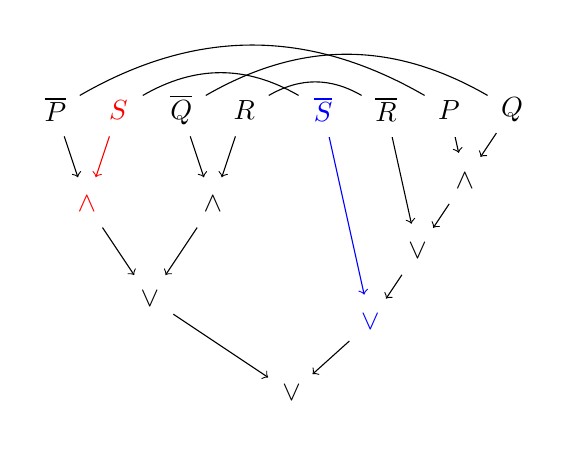
\begin{tikzpicture}
  \tikzstyle{every node}=[circle, minimum size=20pt, inner sep=2pt]
  \draw (0, 0) node (par1) {$\cor$};
  \draw (1, 0.9) node (par3) {\color{blue} $\cor$};
  \draw (-1.8, 1.2) node (par2) {$\cor$};
  \draw (-2.6, 2.4) node (tens1) {\color{red} $\cand$};
  \draw (-1, 2.4) node (tens2) {$\cand$};
  \draw (-2.2, 3.6) node (S) {\color{red} $S$};
  \draw (-0.6, 3.6) node (R) {$R$};
  \draw (-3, 3.6) node (nP) {$\overline{P}$};
  \draw (-1.4, 3.6) node (nQ) {$\overline{Q}$};
  \draw (0.4, 3.6) node (nS) {\color{blue} $\overline{S}$};
  \draw (1.6, 1.8) node (par4) {$\cor$};
  \draw (2.2, 2.7) node (tens3) {$\cand$};
  \draw (2, 3.6) node (P) {$P$};
  \draw (2.8, 3.6) node (Q) {$Q$};
  \draw (1.2, 3.6) node (nR) {$\overline{R}$};
  \draw (par2) -- (par1) [->];
  \draw (par3) -- (par1) [->];
  \draw (tens1) -- (par2) [->];
  \draw (tens2) -- (par2) [->];
  \draw (nP) -- (tens1) [->];
  \draw (S) -- (tens1) [->, color=red];
  \draw (nQ) -- (tens2) [->];
  \draw (R) -- (tens2) [->];
  \draw (nS) -- (par3) [->, color=blue];
  \draw (nR) -- (par4) [->];
  \draw (tens3) -- (par4) [->];
  \draw (P) -- (tens3) [->];
  \draw (Q) -- (tens3) [->];
  \draw (par4) -- (par3) [->];
  \draw (nP) to [bend left] (P);
  \draw (nQ) to [bend left] (Q);
  \draw (S) to [bend left] (nS);
  \draw (R) to [bend left] (nR);
\end{tikzpicture}

\caption{A unification net and its frame. The colored part shows how the
dependency ${\color{red} \exists x} \rightarrow {\color{blue} \forall z}$ is
transformed.}
\end{center}
\end{figure}

We have the following results: 

Let $u$ and $v$ be atoms or quantifiers in a unification structure $\theta$. Then they are connected by a switching path in the unification structure if, and only if, their corresponding nodes are connected by a switching path in $\theta_m$.

Consider now a switching graph $H$ of a unification structure $\theta$ of $A$.

If $H$ contains a cycle, then the corresponding switching graph of $\theta_m$
also contains a cycle. Hence, by applying the propositional results (Theorem 7)
from \cite{retore:03}, we conclude that there exists a chordless, alternating, and elementary cycle in the bicoloured graph ($W, E_W \uplus L_W$), which corresponds to an induced bimatching in the linked fograph. (Note that the linked fograph (cograph) corresponding to $\theta_m$ is equivalent to the one corresponding to $\theta$.)

\end{proof}
\end{proposition}

\subsection{From contraction/weakening to skew bifibrations}

We first introduce the atomic contraction rule, the medial rule, and two rules
on quantifiers.

\begin{center}
\begin{prooftree}
  \hypo{\vdash S\{a \cor a\}}
  \infer1[$\acD$]{\vdash S\{a\}}
\end{prooftree}
\qquad
\begin{prooftree}
  \hypo{\vdash S\{(A \cand B) \cor (C \cand D)\}}
  \infer1[$\me$]{\vdash S\{(A \cor C) \cand (B \cor D)\}}
\end{prooftree}
\\[1.5ex]
\begin{prooftree}
  \hypo{\vdash S\{\exists x A \cor \exists x B\}}
  \infer1[$\mee$]{\vdash S\{\exists x (A \cor B)\}}
\end{prooftree}	
\qquad
\begin{prooftree}
  \hypo{\vdash S\{\forall x A \cor \forall x B\}}
  \infer1[$\meee$]{\vdash S\{\forall x (A \cor B)\}}
\end{prooftree}	
\end{center}

Here, we also consider the equivalence generated by the associativity, commutativity of $\cor$ and the equations $\ttt \cor A \equiv \ttt$ and $\fff \cor A \equiv A$.

Now we have the following lemma:

\begin{lemma}
\label{lemma_ctr}
The contraction rule $\cD$ is derivable for $\{\acD, \me, \mee, \meee\}$.
\end{lemma}
\begin{proof}
	We prove that there is always $\vlderivation{\vlde{}{\{\acD, \me, \mee,
	\meee\}}{A}{\vlhy {A \cor A}}}$ by structural induction on $A$.
\begin{itemize}
  \item If $A = \ttt$ or $A = \fff$, we have 
	  \begin{prooftree} 
	    \hypo{\vdash S\{A \cor A\}}
	    \infer1[$\equiv$]{\vdash S\{A\}}
	  \end{prooftree}. (the premiss and the conclusion are equivalent)
  \item If $A = a$, then we have 
	  \begin{prooftree}
	    \hypo{\vdash S\{a \cor a\}}
	    \infer1[$\acD$]{\vdash S\{a\}}.
	  \end{prooftree}
  \item If $A = A_1 \cor A_2$, then by the induction hypothesis, we have 
	  $\vlderivation{\vlde{}{\{\acD, \me, \mee,
	\meee\}}{A_i}{\vlhy {A_i \cor A_i}}}$ for $i = 1, 2$.
	
	Hence, we have
	\begin{prooftree}
	  \hypo{\vdash S\{(A_1 \cor A_2) \cor (A_1 \cor A_2)\}}
	  \infer1[$\equiv$]{\vdash S\{(A_1 \cor A_1) \cor (A_2 \cor A_2)\}}
	  \ellipsis{$\{\acD, \me, \mee, \meee\}$}
		   {\vdash S\{A_1 \cor (A_2 \cor A_2)\}}
	  \ellipsis{$\{\acD, \me, \mee, \meee\}$}
		   {\vdash S\{A_1 \cor A_2\}}
	\end{prooftree}
  \item If $A = A_1 \cand A_2$, then by the induction hypothesis, we have 
$\vlderivation{\vlde{}{\{\acD, \me, \mee, \meee\}}{A_i}
	      {\vlhy {A_i \cor A_i}}}$ for $i = 1, 2$.

 	Hence, we have
	\begin{prooftree}
	  \hypo{\vdash S\{(A_1 \cand A_2) \cor (A_1 \cand A_2)\}}
	  \infer1[$\me$]{\vdash S\{(A_1 \cor A_1) \cand (A_2 \cor A_2)\}}
	  \ellipsis{$\{\acD, \me, \mee, \meee\}$}
		   {\vdash S\{A_1 \cand (A_2 \cor A_2)\}}
	  \ellipsis{$\{\acD, \me, \mee, \meee\}$}
		   {\vdash S\{A_1 \cand A_2\}}
	\end{prooftree}
  \item If $A = \exists x A'$, then by the induction hypothesis, we have $\vlderivation{\vlde{}{\{\acD, \me, \mee,
	\meee\}}{A'}{\vlhy {A' \cor A'}}}$.

	Hence, we have
	\begin{prooftree}
	  \hypo{\vdash S\{\exists x A' \cor \exists x A'\}}
 	  \infer1[$\mee$]{\vdash S\{\exists x (A' \cor A')\}}
	  \ellipsis{$\{\acD, \me, \mee, \meee\}$}
		   {\vdash S\{\exists x A'\}}
	\end{prooftree}
  \item If $A = \forall x A'$, then by the induction hypothesis, we have $\vlderivation{\vlde{}{\{\acD, \me, \mee,
	\meee\}}{A'}{\vlhy {A' \cor A'}}}$.

	Hence, we have
	\begin{prooftree}
	  \hypo{\vdash S\{\forall x A' \cor \forall x A'\}}
 	  \infer1[$\meee$]{\vdash S\{\forall x (A' \cor A')\}}
	  \ellipsis{$\{\acD, \me, \mee, \meee\}$}
		   {\vdash S\{\forall x A'\}}
	\end{prooftree}

\end{itemize}

\end{proof}

\begin{lemma}
The rules $\mee$ and $\meee$ are derivable for $\{\wD, \cD\}$.
\end{lemma}

\begin{proof}
We have:
\begin{center}
\begin{prooftree}
  \hypo{\vdash S\{\exists x A\}}
  \infer1[$\equiv$]{\vdash S\{\exists x (A \cor \fff)\}}
  \infer1[$\wD$]{\vdash S\{\exists x (A \cor B)\}}
\end{prooftree}
\hspace{0.5cm}
and 
\hspace{0.5cm}
\begin{prooftree}
  \hypo{\vdash S\{\exists x B\}}
  \infer1[$\equiv$]{\vdash S\{\exists x (\fff \cor B)\}}
  \infer1[$\wD$]{\vdash S\{\exists x (A \cor B)\}}
\end{prooftree}
\end{center}
Thus, we have:

\begin{center}
\begin{prooftree}
  \hypo{\vdash S\{\exists x A \cor \exists x B\}}
  \ellipsis{}{\vdash S\{\exists x (A \cor B) \cor \exists x (A \cor B)\}}
  \infer1[$\cD$]{\vdash S\{\exists x (A \cor B)\}}
\end{prooftree}
\end{center}
Similar for $\meee$.
\end{proof}

Now we define a propositional encoding for first-order formulas.

\begin{definition}
The propositional encoding $\PE{A}$ of a formula $A$ is defined inductively by:

\begin{centering}
	$\PE{a} = a$ for every atom $a$

	$\PE{(A \cor B)} = \PE{A} \cor \PE{B}$ \hspace{2cm} $\PE{(A \cand B)} =
	\PE{A} \cand \PE{B}$

	$\PE{(\forall x A)} = U_x \cor \PE{A}$ \hspace{2cm} $\PE{(\exists x A)}
	= E_x \cand \PE{A}$

\end{centering}
where $U_x$ and $E_x$ are fresh nullary atoms.

\end{definition}

Similarly, we can define the propositional encoding $\PE{S}$ of a context $S$
inductively by setting $\PE{\Box} = \Box$. Note that $\PE{S}$ is also a context.

We have the following facts:

\begin{proposition}
For any context $S$ and any formula $A$:
\begin{itemize}
  \item $\PE{A}$ is a formula containing no quantifier for any formula $A$.
  \item $\graphof(\PE{A}) = \graphof(A)$ by confounding the atoms $U_x$, $E_x$ with the variable
	  $x$. Thus, a map $f : \graphof(\PE{A}) \rightarrow \graphof(\PE{B})$ can be seen as a map
		$f : \graphof(A) \rightarrow \graphof(B)$.
  \item $\PE{(S\{A\})} = \PE{S}\{\PE{A}\}$.
\end{itemize}

\end{proposition}

\begin{proposition}
\label{prop311}
Let $A$ and $B$ be two formulas such that
$\od{\odd{\odh {A}}{}{B}{\{\wD, \cD\}}}$. Then 
$\od{\odd{\odh {\PE{A}}}{}{\PE{B}}{\{\wD, \cD\}}}$.
\end{proposition}
\begin{proof}
  Trivial by induction.
\end{proof}

\begin{lemma}
\label{mlem}
	Given two formulas $A$ and $B$ and a derivation $\od{\odd{\odh {A}}
	{\Delta}{B}{\{\wD, \cD\}}}$, then there exists a skew bifibration $G(A)
	\rightarrow G(B)$.
\end{lemma}

\begin{proof}
By Lemma \ref{lemma_ctr}, there exists a derivation $\od{\odd{\odh {A}}
	{\Delta}{B}{\{\wD, \acD, \me, \mee, \meee \}}}$.
	
For each rule from $\{\wD, \acD, \me, \mee, \meee \}$, we define a map and show that it is a skew fibration.

\begin{itemize}
  \item \begin{prooftree}
  \hypo{\vdash S\{\fff \}}
  \infer1[$\wD$]{\vdash S\{A\}}
\end{prooftree}:

  the map $wk$ maps $\fff$ to anything and is identity elsewhere.   
 
  \item
    \begin{prooftree}
      \hypo{\vdash S\{a \cor a\}}
       \infer1[$\acD$]{\vdash S\{a\}} 
    \end{prooftree}: 
    
    the map $ac$ maps the two $a$-labelled literals in the premise to the $a$-labelled literal in the conclusion.

  \item 
    \begin{prooftree}
      \hypo{\vdash S\{(A \cand B) \cor (C \cand D)\}}
      \infer1[$\me$]{\vdash S\{(A \cor C) \cand (B \cor D)\}}
    \end{prooftree}:
    
    the map $m$ is the canonical identity that maps $A$ to $A$, $\cdots$, $D$ to $D$.
  \item 
    \begin{prooftree}
      \hypo{\vdash S\{\exists x A \cor \exists x B\}}
      \infer1[$\mee$]{\vdash S\{\exists x (A \cor B)\}}
    \end{prooftree}: 
   
    the map $m_1$ maps the two $x$-labelled binders in the premise to the $x$-labelled binder in the conclusion,  $A$ to $A$ and $B$ to $B$.
  \item
    \begin{prooftree}
      \hypo{\vdash S\{\forall x A \cor \forall x B\}}
      \infer1[$\meee$]{\vdash S\{\forall x (A \cor B)\}}
    \end{prooftree}:
    
    the map $m_2$ maps the two $x$-labelled binders in the premise to the $x$-labelled binder in the conclusion,  $A$ to $A$ and $B$ to $B$. 

\end{itemize}

By considering propositional encodings, the maps defined are label-preserving
skew fibrations on the underlying fographs according to
\cite{str:07:RTA}.

Now we prove that each map $g \in \{wk, ac, m, m_1, m_2 \}$ is a skew bifibration. To do that, it suffices to prove that $g$ is a fibration between the corresponding binding graphs since it is already a skew fibration on the corresponding fographs and it is label-preserving and existential-preserving.
\begin{center}
for each $x$-binder $b$ in $\graphof(\PE{B})$, for each vertex $v \in V(\graphof(\PE{A}))$
such that $g(v)$ is bound by $b$, there exists a unique binder $b'$ such
that $b'$ binds $v$.
\end{center}

\begin{itemize}
  \item $wk$ and $m$ are clearly fibrations: the binding relations of the premise and the conclusion are exactly the same.
  \item $ac$ is a fibration: suppose that $a$ that in the conclusion $a$ is bound by some quantifier $b$ in $S$, then for each of its preimages by $ac$, there exists exactly one binder (in fact, $b$) in $S$ that binds it.
  \item $m_1$ and $m_2$ are fibrations: in the conclusion, for every atom $a$ in $A \cor B$ bound by the $x$-labelled quantifier, $a$ has exactly one preimage and it is bound by the $x$-llabelled quantifier in the premise.
\end{itemize}

  Therefore, all of these maps are skew bifibrations and since skew bifibrations
on fographs compose (Lemma 10.32, \cite{hughes:fopws}), there exists a skew
bifibration from $\graphof(A)$ to $\graphof(B)$.

\end{proof}

\begin{theorem_}
If a formula $A$ is provable in $\LK$, then it has a combinatorial proof.
\end{theorem_}

\begin{proof}
By Theorem \ref{thm1}, there exists a formula $A'$ such that there is a proof
$\Pi$ of $A'$ in $\FOMLL$ and a derivation $D$ from $A'$ to $A$ consisting of
the $\wD$ and $\cD$ rules only. The proof $\Pi$ corresponds to a unique
unification net which is equivalent to the fonet corresponding to $\Pi$, i.e.,
the fograph $\graphof(A')$ together with the links of $\Pi$. By Lemma \ref{mlem}, 
there exists a skew bifibration $\graphof(A') \rightarrow \graphof(A)$. We have thus a
combinatorial proof of $A$.

\end{proof}

\subsection{From skew bifibrations to contraction/weakening}

\begin{theorem_}
Let $A$ and $B$ be two formulas and $f: G(A) \rightarrow G(B)$ a skew bifibration. Then there exists a derivation $\od{\odd{\odh {A}}{\Delta}{B}{\{\wD, \cD\}}}$.
\end{theorem_}

$f$ can be seen as a skew fibration from $G(\PE{A})$ to $G(\PE{B})$, which gives the existence of the propositions $A'$ and $B'$, and of the following derivation:
  \[\od{\odd{\odd{\odd{\odh{\PE{A}} }
  {\Delta }{A'}{\me} }
  {\Delta' }{B'}{\acD} }
  {\Delta''}{\PE{B}}{\wD}} \]

\begin{lemma} there exists $B''$ such that $\PE{B''}$ = $B'$.

\begin{proof}
Consider the dervation $\Delta''$. If some $U_x$ (or $E_x$) is introduced
via weakening, then all the atoms it binds in $\PE{B}$ should also be introduced 
via weakening. In fact, an atom of $\PE{B}$ is introduced via weakening is 
equivalent to the fact that its corresponding vertex is not in the image of $f$. 
Since there is an edge from $U_x$ (resp. $E_x$) to all the literals it binds in the 
binding graph $\overrightarrow{\graphof(B)}$, if one of the atoms is in the image, 
$U_x$ (resp. $E_x$) should also be in the image since $f$ is a fibration on binding graphs.

This means that a such $B''$ can be obtained from $B$ by erasing all the $U_x$ and $E_x$ introduced via weakening and all the atoms they bind.
\end{proof}
\end{lemma}

We introduce new (atomic) symbols $E_x^*$ and $U_x^*$ which are used to
represent disjunctions of $E_x$ and $U_x$ respectiveley.

We define a translation $(\cdot)^*$ inductively by:
\begin{itemize}
  \item $(E_x \cor \cdots \cor E_x)^* = E_x$
  \item $(U_x \cor \cdots \cor U_x)^* = U_x$
  \item structural recursion in all the other cases.
\end{itemize}

Then the derivation:
 \[\od{\odd{\odd{\odh{\PE{A}} }
  {\Delta }{A'}{\me} }
  {\Delta' }{\PE{B''}}{\acD}} \]
can be translated to the derivation:
\[\od{\odd{\odh{(\PE{A})^*} }
{\Delta^* }{(\PE{B''})^*}{}} \]

where $\Delta^*$ is the derivation obtained by replacing all the formulas $F$
with $F^*$ and by applying the following rule transformation:

\begin{center}
\mbox{
\begin{prooftree}
  \hypo{S\{Q_x\}}
  \infer1[$\acD$]{S\{Q_x\}}
\end{prooftree}

$\leadsto$

\begin{prooftree}
  \hypo{S\{Q_x\}}
  \infer1[$=$]{S\{Q_x\}}
\end{prooftree}

}
\vspace{0.4cm}

\mbox{
\begin{prooftree}
  \hypo{S\{(E_x \cand C) \cor (E_x \cand D)\}}
  \infer1[$\me$]{S\{E_x \cand (C \cor D)\}}
\end{prooftree}

$\leadsto$

\begin{prooftree}
  \hypo{S\{(E_x \cand C) \cor (E_x \cand D)\}}
  \infer1[$\me'$]{S\{E_x \cand (C \cor D)\}}
\end{prooftree}

}
	
\end{center}
where $Q_x$ stands for $E_x$ or $U_x$.

$\Delta^*$ can now be transformed into a valid derivation $\Delta_1$ by using the two
transformation rules above and by applying them in a bottom-up style:
\[\od{\odd{\odh{(\PE{A})^*} }
{\Delta_1 }{(\PE{B''})^*}{\acD, \me, \me'}} \]

\begin{lemma}
Every line of $\Delta_1$ is a propositional encoding.

\begin{proof}
We proceed by bottom-up induction in the derivation.
Clearly, $(\PE{B''})^*$ is a propositional encoding as there is no disjunction of $Q_x$
in it.

First consider the $\acD$ rule:
\begin{prooftree}
  \hypo{C \cor C}
  \infer1[$\acD$]{C}
\end{prooftree}

It is clear that if $C$ is a propositional encoding, then so is $C \cor C$.

Now consider the $\me$ rule:
\begin{center}
\begin{prooftree}
  \hypo{S\{(C \cand D) \cor (E \cand F)\}}
  \infer1[$\me$]{S\{(C \cor E) \cand (D \cor F)\}}
\end{prooftree}
\end{center}
Suppose that $(C \cor E) \cand (D \cor F) = \PE{G}$ for some $G$.
Since $C \cor E$ cannot be $Q_x$ (otherwise, the rule applied would be
$\me'$), $G$ can be written as $G_1 \cand G_2$ with $C \cor E = \PE{G_1}$ and $D
\cor F = \PE{G_2}$.

We have thus $G_i = \forall x_i H_i$ or $J_i \cor K_i (i = 1, 2)$.

If $G_i = \forall x H_i$ for some $i$, then there will be a conjunction of $U_x$
and some formula which can never be eliminated by the rules $\me$, $\me'$ and
$\acD$. However, there exists no such conjunction in ${\PE{A}}^*$, which leads to a
contradiction.

Hence, $G_i$ can be written as $J_i \cor K_i$ for $i = 1, 2$. We now have $(C
\cand D) \cor (E \cand F) = \PE{((J_1 \cand J_2) \cor (K_1 \cand
K_2))}$.

Finally, consider the $\me'$ rule:
\begin{center}
\begin{prooftree}
  \hypo{S\{(E_x \cand C) \cor (E_x \cand D)\}}
  \infer1[$\me'$]{S\{E_x \cand (C \cor D)\}}
\end{prooftree}
\end{center}
Suppose that $E_X \cand (C \cor D)$ = $\PE{F}$ for some $F$. It is clear
that $F = \exists x G$ with $\PE{G} = C \cor D$ for some $G$.
We distinguish two cases:
\begin{itemize}
  \item $G = \forall y H$: in this case, $(E_x \cand C) \cor (E_x \cand
D)$ has a subformula $(E_x \cand U_y)$, which cannot be eliminated by the
	rules $\me$, $\me'$, $\acD$. It is clear that ${\PE{A}}^*$ does not
have a subformula of this form, which leads to a contradiction.
  \item $G = G_1 \cor G_2$: in this case, $(E_x \cand C) \cor (E_x \cand
  D) = \PE{((\exists x G_1) \cor (\exists x G_2))}$.
\end{itemize}

\end{proof}	
\end{lemma}

% An example of a floating figure using the graphicx package.
% Note that \label must occur AFTER (or within) \caption.
% For figures, \caption should occur after the \includegraphics.
% Note that IEEEtran v1.7 and later has special internal code that
% is designed to preserve the operation of \label within \caption
% even when the captionsoff option is in effect. However, because
% of issues like this, it may be the safest practice to put all your
% \label just after \caption rather than within \caption{}.
%
% Reminder: the "draftcls" or "draftclsnofoot", not "draft", class
% option should be used if it is desired that the figures are to be
% displayed while in draft mode.
%
%\begin{figure}[!t]
%\centering
%\includegraphics[width=2.5in]{myfigure}
% where an .eps filename suffix will be assumed under latex, 
% and a .pdf suffix will be assumed for pdflatex; or what has been declared
% via \DeclareGraphicsExtensions.
%\caption{Simulation results for the network.}
%\label{fig_sim}
%\end{figure}

% Note that the IEEE typically puts floats only at the top, even when this
% results in a large percentage of a column being occupied by floats.


% An example of a double column floating figure using two subfigures.
% (The subfig.sty package must be loaded for this to work.)
% The subfigure \label commands are set within each subfloat command,
% and the \label for the overall figure must come after \caption.
% \hfil is used as a separator to get equal spacing.
% Watch out that the combined width of all the subfigures on a 
% line do not exceed the text width or a line break will occur.
%
%\begin{figure*}[!t]
%\centering
%\subfloat[Case I]{\includegraphics[width=2.5in]{box}%
%\label{fig_first_case}}
%\hfil
%\subfloat[Case II]{\includegraphics[width=2.5in]{box}%
%\label{fig_second_case}}
%\caption{Simulation results for the network.}
%\label{fig_sim}
%\end{figure*}
%
% Note that often IEEE papers with subfigures do not employ subfigure
% captions (using the optional argument to \subfloat[]), but instead will
% reference/describe all of them (a), (b), etc., within the main caption.
% Be aware that for subfig.sty to generate the (a), (b), etc., subfigure
% labels, the optional argument to \subfloat must be present. If a
% subcaption is not desired, just leave its contents blank,
% e.g., \subfloat[].


% An example of a floating table. Note that, for IEEE style tables, the
% \caption command should come BEFORE the table and, given that table
% captions serve much like titles, are usually capitalized except for words
% such as a, an, and, as, at, but, by, for, in, nor, of, on, or, the, to
% and up, which are usually not capitalized unless they are the first or
% last word of the caption. Table text will default to \footnotesize as
% the IEEE normally uses this smaller font for tables.
% The \label must come after \caption as always.
%
%\begin{table}[!t]
%% increase table row spacing, adjust to taste
%\renewcommand{\arraystretch}{1.3}
% if using array.sty, it might be a good idea to tweak the value of
% \extrarowheight as needed to properly center the text within the cells
%\caption{An Example of a Table}
%\label{table_example}
%\centering
%% Some packages, such as MDW tools, offer better commands for making tables
%% than the plain LaTeX2e tabular which is used here.
%\begin{tabular}{|c||c|}
%\hline
%One & Two\\
%\hline
%Three & Four\\
%\hline
%\end{tabular}
%\end{table}


% Note that the IEEE does not put floats in the very first column
% - or typically anywhere on the first page for that matter. Also,
% in-text middle ("here") positioning is typically not used, but it
% is allowed and encouraged for Computer Society conferences (but
% not Computer Society journals). Most IEEE journals/conferences use
% top floats exclusively. 
% Note that, LaTeX2e, unlike IEEE journals/conferences, places
% footnotes above bottom floats. This can be corrected via the
% \fnbelowfloat command of the stfloats package.




\section{Conclusion}





% conference papers do not normally have an appendix


% use section* for acknowledgment
%\section*{Acknowledgment}


%The authors would like to thank...





% trigger a \newpage just before the given reference
% number - used to balance the columns on the last page
% adjust value as needed - may need to be readjusted if
% the document is modified later
%\IEEEtriggeratref{8}
% The "triggered" command can be changed if desired:
%\IEEEtriggercmd{\enlargethispage{-5in}}

% references section

% can use a bibliography generated by BibTeX as a .bbl file
% BibTeX documentation can be easily obtained at:
% http://mirror.ctan.org/biblio/bibtex/contrib/doc/
% The IEEEtran BibTeX style support page is at:
% http://www.michaelshell.org/tex/ieeetran/bibtex/
%\bibliographystyle{IEEEtran}
% argument is your BibTeX string definitions and bibliography database(s)
%\bibliography{IEEEabrv,../bib/paper}
%
% <OR> manually copy in the resultant .bbl file
% set second argument of \begin to the number of references
% (used to reserve space for the reference number labels box)

\bibliographystyle{IEEEtran}
\bibliography{refs}

%\begin{thebibliography}{1}

%\bibitem{IEEEhowto:kopka}
%H.~Kopka and P.~W. Daly, \emph{A Guide to \LaTeX}, 3rd~ed.\hskip 1em plus
%  0.5em minus 0.4em\relax Harlow, England: Addison-Wesley, 1999.

%\end{thebibliography}




% that's all folks
\end{document}

